% Options for packages loaded elsewhere
\PassOptionsToPackage{unicode}{hyperref}
\PassOptionsToPackage{hyphens}{url}
\PassOptionsToPackage{dvipsnames,svgnames,x11names}{xcolor}
%
\documentclass[
  english,
  man,floatsintext]{apa6}
\title{Descriptive, not injunctive, social norms caused increases in mask wearing throughout the COVID-19 pandemic}
\author{Samantha L. Heiman\textsuperscript{$\dagger{}$,1}, Scott Claessens\textsuperscript{$\dagger{}$,2}, Edward R. Hurt\textsuperscript{1}, \& Peter M. Todd\textsuperscript{1,3}}
\date{}

\usepackage{amsmath,amssymb}
\usepackage{lmodern}
\usepackage{iftex}
\ifPDFTeX
  \usepackage[T1]{fontenc}
  \usepackage[utf8]{inputenc}
  \usepackage{textcomp} % provide euro and other symbols
\else % if luatex or xetex
  \usepackage{unicode-math}
  \defaultfontfeatures{Scale=MatchLowercase}
  \defaultfontfeatures[\rmfamily]{Ligatures=TeX,Scale=1}
\fi
% Use upquote if available, for straight quotes in verbatim environments
\IfFileExists{upquote.sty}{\usepackage{upquote}}{}
\IfFileExists{microtype.sty}{% use microtype if available
  \usepackage[]{microtype}
  \UseMicrotypeSet[protrusion]{basicmath} % disable protrusion for tt fonts
}{}
\makeatletter
\@ifundefined{KOMAClassName}{% if non-KOMA class
  \IfFileExists{parskip.sty}{%
    \usepackage{parskip}
  }{% else
    \setlength{\parindent}{0pt}
    \setlength{\parskip}{6pt plus 2pt minus 1pt}}
}{% if KOMA class
  \KOMAoptions{parskip=half}}
\makeatother
\usepackage{xcolor}
\IfFileExists{xurl.sty}{\usepackage{xurl}}{} % add URL line breaks if available
\IfFileExists{bookmark.sty}{\usepackage{bookmark}}{\usepackage{hyperref}}
\hypersetup{
  pdftitle={Descriptive, not injunctive, social norms caused increases in mask wearing throughout the COVID-19 pandemic},
  pdfauthor={Samantha L. Heiman,1, Scott Claessens,2, Edward R. Hurt1, \& Peter M. Todd1,3},
  pdflang={en-EN},
  pdfkeywords={descriptive norms; injunctive norms; longitudinal; COVID-19; mask wearing; cooperation},
  colorlinks=true,
  linkcolor={Maroon},
  filecolor={Maroon},
  citecolor={Blue},
  urlcolor={blue},
  pdfcreator={LaTeX via pandoc}}
\urlstyle{same} % disable monospaced font for URLs
\usepackage{graphicx}
\makeatletter
\def\maxwidth{\ifdim\Gin@nat@width>\linewidth\linewidth\else\Gin@nat@width\fi}
\def\maxheight{\ifdim\Gin@nat@height>\textheight\textheight\else\Gin@nat@height\fi}
\makeatother
% Scale images if necessary, so that they will not overflow the page
% margins by default, and it is still possible to overwrite the defaults
% using explicit options in \includegraphics[width, height, ...]{}
\setkeys{Gin}{width=\maxwidth,height=\maxheight,keepaspectratio}
% Set default figure placement to htbp
\makeatletter
\def\fps@figure{htbp}
\makeatother
\setlength{\emergencystretch}{3em} % prevent overfull lines
\providecommand{\tightlist}{%
  \setlength{\itemsep}{0pt}\setlength{\parskip}{0pt}}
\setcounter{secnumdepth}{-\maxdimen} % remove section numbering
% Make \paragraph and \subparagraph free-standing
\ifx\paragraph\undefined\else
  \let\oldparagraph\paragraph
  \renewcommand{\paragraph}[1]{\oldparagraph{#1}\mbox{}}
\fi
\ifx\subparagraph\undefined\else
  \let\oldsubparagraph\subparagraph
  \renewcommand{\subparagraph}[1]{\oldsubparagraph{#1}\mbox{}}
\fi
\newlength{\cslhangindent}
\setlength{\cslhangindent}{1.5em}
\newlength{\csllabelwidth}
\setlength{\csllabelwidth}{3em}
\newlength{\cslentryspacingunit} % times entry-spacing
\setlength{\cslentryspacingunit}{\parskip}
\newenvironment{CSLReferences}[2] % #1 hanging-ident, #2 entry spacing
 {% don't indent paragraphs
  \setlength{\parindent}{0pt}
  % turn on hanging indent if param 1 is 1
  \ifodd #1
  \let\oldpar\par
  \def\par{\hangindent=\cslhangindent\oldpar}
  \fi
  % set entry spacing
  \setlength{\parskip}{#2\cslentryspacingunit}
 }%
 {}
\usepackage{calc}
\newcommand{\CSLBlock}[1]{#1\hfill\break}
\newcommand{\CSLLeftMargin}[1]{\parbox[t]{\csllabelwidth}{#1}}
\newcommand{\CSLRightInline}[1]{\parbox[t]{\linewidth - \csllabelwidth}{#1}\break}
\newcommand{\CSLIndent}[1]{\hspace{\cslhangindent}#1}
% Manuscript styling
\usepackage{upgreek}
\captionsetup{font=singlespacing,justification=justified}

% Table formatting
\usepackage{longtable}
\usepackage{lscape}
% \usepackage[counterclockwise]{rotating}   % Landscape page setup for large tables
\usepackage{multirow}		% Table styling
\usepackage{tabularx}		% Control Column width
\usepackage[flushleft]{threeparttable}	% Allows for three part tables with a specified notes section
\usepackage{threeparttablex}            % Lets threeparttable work with longtable

% Create new environments so endfloat can handle them
% \newenvironment{ltable}
%   {\begin{landscape}\centering\begin{threeparttable}}
%   {\end{threeparttable}\end{landscape}}
\newenvironment{lltable}{\begin{landscape}\centering\begin{ThreePartTable}}{\end{ThreePartTable}\end{landscape}}

% Enables adjusting longtable caption width to table width
% Solution found at http://golatex.de/longtable-mit-caption-so-breit-wie-die-tabelle-t15767.html
\makeatletter
\newcommand\LastLTentrywidth{1em}
\newlength\longtablewidth
\setlength{\longtablewidth}{1in}
\newcommand{\getlongtablewidth}{\begingroup \ifcsname LT@\roman{LT@tables}\endcsname \global\longtablewidth=0pt \renewcommand{\LT@entry}[2]{\global\advance\longtablewidth by ##2\relax\gdef\LastLTentrywidth{##2}}\@nameuse{LT@\roman{LT@tables}} \fi \endgroup}

% \setlength{\parindent}{0.5in}
% \setlength{\parskip}{0pt plus 0pt minus 0pt}

% Overwrite redefinition of paragraph and subparagraph by the default LaTeX template
% See https://github.com/crsh/papaja/issues/292
\makeatletter
\renewcommand{\paragraph}{\@startsection{paragraph}{4}{\parindent}%
  {0\baselineskip \@plus 0.2ex \@minus 0.2ex}%
  {-1em}%
  {\normalfont\normalsize\bfseries\itshape\typesectitle}}

\renewcommand{\subparagraph}[1]{\@startsection{subparagraph}{5}{1em}%
  {0\baselineskip \@plus 0.2ex \@minus 0.2ex}%
  {-\z@\relax}%
  {\normalfont\normalsize\itshape\hspace{\parindent}{#1}\textit{\addperi}}{\relax}}
\makeatother

% \usepackage{etoolbox}
\makeatletter
\patchcmd{\HyOrg@maketitle}
  {\section{\normalfont\normalsize\abstractname}}
  {\section*{\normalfont\normalsize\abstractname}}
  {}{\typeout{Failed to patch abstract.}}
\patchcmd{\HyOrg@maketitle}
  {\section{\protect\normalfont{\@title}}}
  {\section*{\protect\normalfont{\@title}}}
  {}{\typeout{Failed to patch title.}}
\makeatother

\usepackage{xpatch}
\makeatletter
\xapptocmd\appendix
  {\xapptocmd\section
    {\addcontentsline{toc}{section}{\appendixname\ifoneappendix\else~\theappendix\fi\\: #1}}
    {}{\InnerPatchFailed}%
  }
{}{\PatchFailed}
\keywords{descriptive norms; injunctive norms; longitudinal; COVID-19; mask wearing; cooperation\newline\indent Word count: 4826 words}
\usepackage{lineno}

\linenumbers
\usepackage{csquotes}
\usepackage{array}
\usepackage{caption}
\usepackage{graphicx}
\usepackage{siunitx}
\usepackage[normalem]{ulem}
\usepackage{colortbl}
\usepackage{multirow}
\usepackage{hhline}
\usepackage{calc}
\usepackage{tabularx}
\usepackage{threeparttable}
\usepackage{wrapfig}
\usepackage{adjustbox}
\usepackage{hyperref}
\usepackage{setspace}
\raggedbottom
\AtBeginEnvironment{tabular}{\singlespacing}
\AtBeginEnvironment{lltable}{\singlespacing}
\AtBeginEnvironment{tablenotes}{\doublespacing}
\captionsetup[table]{font={stretch=1,small}}
\captionsetup[figure]{font={stretch=1,small}}
\ifXeTeX
  % Load polyglossia as late as possible: uses bidi with RTL langages (e.g. Hebrew, Arabic)
  \usepackage{polyglossia}
  \setmainlanguage[]{english}
\else
  \usepackage[main=english]{babel}
% get rid of language-specific shorthands (see #6817):
\let\LanguageShortHands\languageshorthands
\def\languageshorthands#1{}
\fi
\ifLuaTeX
  \usepackage{selnolig}  % disable illegal ligatures
\fi


\shorttitle{Norms and mask wearing}

\authornote{

\textsuperscript{$\dagger{}$} Samantha L. Heiman and Scott Claessens contributed equally to this work.

Correspondence concerning this article should be addressed to Peter M. Todd, 1101 E 10th St, Bloomington, IN 47405, United States. E-mail: \href{mailto:pmtodd@indiana.edu}{\nolinkurl{pmtodd@indiana.edu}}

}

\affiliation{\vspace{0.5cm}\textsuperscript{1} Department of Psychological and Brain Sciences, Indiana University Bloomington, United States\\\textsuperscript{2} School of Psychology, University of Auckland, New Zealand\\\textsuperscript{3} Cognitive Science Program, Indiana University Bloomington, United States}

\note{This working paper has not yet been peer-reviewed. This study was funded by the Interdisciplinary Cooperation Initiative, ASU President's Office, the Cooperation Science Network, the Institute for Mental Health Research, the University of New Mexico, the Indiana University College of Arts \& Sciences, the Rutgers University Center for Human Evolutionary Studies, the Charles Koch Foundation, and the John Templeton Foundation.}

\abstract{%
Social norms allow humans to coordinate and cooperate in the face of existential threats. In particular, injunctive social norms prescribe what people \emph{ought} to do, whereas descriptive social norms inform what people \emph{actually} do. While previous experimental work has revealed people's sensitivity to normative influence, several open questions remain about the natural emergence of injunctive and descriptive social norms within populations and their influences on cooperative behavior over time. To understand how social norms emerge and shape behavior in a non-experimental setting, we studied mask wearing during the COVID-19 pandemic. Leveraging a year and a half of longitudinal data from a representative sample of adults in the United States (15 time points; \emph{n} = 915), we tracked people's reported mask wearing behavior and their perceived injunctive and descriptive mask wearing norms as the pandemic unfolded. Longitudinal trends of norm perceptions and self-reported mask wearing suggested that norms and behavior are tightly coupled and both change quickly in response to recommendations from public health authorities. In addition, a random-intercept cross-lagged panel model revealed that descriptive norms, but not injunctive norms, caused future increases in mask wearing behavior. These findings underline the relative importance of descriptive social norms in shaping cooperative behavior during uncertain times.
}



\begin{document}
\maketitle

Social norms are a key aspect of human sociality. Broadly defined as behavioral guidelines enforced by groups of people without the law (van Kleef et al., 2019), social norms have attracted the attention of psychologists for decades. Since Asch's (1956) early studies of normative conformity, evidence has accrued that humans are particularly attuned to social norms (Tomasello, 2014). From a young age, children begin to adhere to and enforce group-wide social norms (Jensen et al., 2014; Rakoczy \& Schmidt, 2013; Schmidt \& Tomasello, 2012) and both children and adults rely on normative emotions, such as shame and guilt, to determine when they or others have violated social norms (Schaumberg \& Skowronek, 2022; Vaish et al., 2011). This uniquely human sensitivity to social norms allows groups of unrelated people to cooperate and coordinate in the face of existential threats, such as resource scarcity, natural disasters, and infectious diseases (Gelfand et al., 2011; Henrich, 2015).

Previous research has distinguished between two primary kinds of social norms: injunctive norms and descriptive norms (Cialdini et al., 1991; Deutsch \& Gerard, 1955). Injunctive social norms are societal, indicating what others in the group tend to approve or disapprove of, and often involve social sanctions if violated. By contrast, descriptive norms are situational, simply describing what most people are doing in a given situation. Though these two kinds of social norms tend to align, they can also be in conflict with one another. For example, there may be an injunctive norm that cleaning up litter at a picnic site is the right thing to do: one \emph{ought} to behave this way. However, if an individual observes that most people are leaving their litter behind at the site, the descriptive norm is to not clean up. It is thus possible for injunctive and descriptive norms to have independent effects on behavior (Schultz et al., 2007).

Despite decades of research on the causes and consequences of injunctive and descriptive norms (Cialdini et al., 1991; Cialdini, 2007; Cialdini \& Jacobson, 2021; Schultz et al., 2007), social norms have remained an elusive concept in the behavioral sciences and several open questions remain (Fehr \& Schurtenberger, 2018a; van Kleef et al., 2019). In the current work, we focus on two such questions. First, how do injunctive and descriptive norms emerge naturally over time within a population? Second, how do evolving injunctive and descriptive norms influence behavior?

With regards to norm emergence, research in cultural evolution and behavioral economics have begun to illuminate how social norms emerge over time. In the longer term, cultural evolutionary models show that injunctive social norms can be vertically transmitted down through generations via imitation or teaching, or horizontally diffused from neighboring human populations (Boyd, 1985; Henrich, 2015). For example, cultural phylogenetic studies have revealed patterns of vertical cultural inheritance across societies for a variety of injunctive social norms, such as norms governing land ownership (Kushnick et al., 2014) and post-marital residence (Jordan et al., 2009). However, much less is known about how social norms arise endogenously within populations in the shorter term. Recent experimental work in behavioral economics suggests that social norms of public good provisioning develop in tandem with cooperative behavior through repeated interactions (Titlestad et al., 2019) and require peer enforcement to become stable (Fehr \& Schurtenberger, 2018b). But it remains unclear to what extent these findings generalize beyond the laboratory to real human populations.

With regards to normative influences on behavior, there is a wealth of cross-sectional evidence demonstrating the behavioral impact of social norms. For example, field experiments have demonstrated the positive effects of descriptive norms on a variety of cooperative behaviors, including recycling (Nigbur et al., 2010), paying taxes (Larkin et al., 2018), and sustainably reusing towels in hotels (Goldstein et al., 2008). Evidence also suggests that any potentially deleterious effects of descriptive social norms (e.g., choosing to litter at a picnic site that already contains visible signs of littering) can be counteracted by instead focusing individuals' attention on injunctive norms (Schultz et al., 2007). However, previous studies have tended to follow experimental designs in which perceptions of social norms are manipulated by the researchers, and thus do not allow cooperative social norms to emerge and affect behavior naturally over time within a population. An alternative way to identify causality, whilst retaining ecological validity, is to follow perceptions of social norms and cooperative behavior over time amidst a real, unfolding social dilemma. This is particularly important because social norms are not static: they change dynamically over time through processes of deliberation and social interaction (Smith et al., 2015).

To understand how novel injunctive and descriptive social norms emerge over time and shape cooperative behavior in a non-experimental setting, we studied mask wearing behavior during the COVID-19 pandemic. Before the pandemic, mask wearing was not a common behavior in the United States. In April 2020, two months into the pandemic, mask wearing was officially recommended by the Centers for Disease Control and Prevention (CDC) as a measure that people should take to minimize the spread of COVID-19. But mask wearing posed a social dilemma to individuals, in that it imposed personal costs (e.g., difficulty breathing, disrupted social interaction) for the benefit of the wider community (e.g., ``flattening the curve'' to protect at-risk individuals). Thus, the evolution of mask wearing in the United States throughout the COVID-19 pandemic allows us to study, on a short timescale within a single population, the emergence of novel injunctive and descriptive social norms and the causal effects of these norms on cooperative behavior.

Recent research has found positive relationships between perceptions of social norms and protective COVID-19 behaviors. In the United States, one cross-sectional study found that perceptions of injunctive norms positively predicted intentions to stay at home to minimize exposure (Macy et al., 2021), and another vignette study found that experimentally-manipulated descriptive norms increased personal mask wearing intentions (Bokemper et al., 2021). In Germany, a two-wave study found that perceptions of descriptive norms positively predicted future protective behaviors, such as physical distancing (Rudert \& Janke, 2021). These studies are telling, but since they are experimental, cross-sectional, or only minimally longitudinal, they are unable to distinguish between between-person and within-person change over time (Hamaker et al., 2015), nor do they have the temporal granularity to capture fluctuating changes in norm strength and norm adherence across the entire pandemic.

Here, we use a year and a half of longitudinal data from a representative sample of adults in the United States (15 time points; \emph{n} = 916) to track the development of descriptive and injunctive mask wearing norms and mask wearing behavior over the course of the COVID-19 pandemic. We aimed to answer two main research questions. First, how do descriptive and injunctive mask wearing norms emerge and evolve over time in the United States population? Second, how do descriptive and injunctive mask wearing norms affect mask wearing behavior over time?

\hypertarget{methods}{%
\section{Methods}\label{methods}}

\hypertarget{ethical-approval}{%
\subsection{Ethical approval}\label{ethical-approval}}

This project was granted exemption from the Institutional Review Board of Arizona State University (STUDY00011678). All participants in this study provided informed consent.

\hypertarget{participants-and-sampling}{%
\subsection{Participants and sampling}\label{participants-and-sampling}}

Using the platform Prolific (\url{https://www.prolific.co/}), we distributed surveys to a representative sample of adults from the United States (\emph{n} = 915, \emph{M}\textsubscript{age} = 46 years, 75\% White, 52\% Women; see Supplementary Figure \ref{fig:plotUSMap} for geographic distribution). From September 2020 to February 2022, we asked participants to complete regular surveys of COVID-19 related attitudes and behaviors. This resulted in 15 unique time points of data collection throughout the pandemic. The first 12 time points were distributed monthly, while the last three time points were distributed every two months. 634 of the initial 915 participants returned to complete the survey at Time 2, while 379 participants continued through to Time 15 (see Supplementary Figure \ref{fig:plotAttrition} for attrition rates across all time points).

\hypertarget{measures}{%
\subsection{Measures}\label{measures}}

\hypertarget{self-reported-mask-wearing-behavior}{%
\subsubsection{Self-reported mask wearing behavior}\label{self-reported-mask-wearing-behavior}}

At every time point, participants were asked about the number of in-person interactions they had in the last week. Following this question, participants self-reported their mask wearing behavior by answering: ``\emph{During these in-person interactions, if you were closer than 6 feet (2 meters) from the person(s) did you wear a face mask?}'' Participants responded on a 5-point Likert scale, from Never (1) to Always (5).

\hypertarget{perceived-descriptive-and-injunctive-social-norms}{%
\subsubsection{Perceived descriptive and injunctive social norms}\label{perceived-descriptive-and-injunctive-social-norms}}

In 8 of the 15 time points (Time 2, 3, 5, 9, 11, 13, 14, and 15), we asked questions about perceived descriptive and injunctive mask wearing norms.

Descriptive social norms were operationalized as the proportion of individuals in participants' local areas wearing masks in routine and recreational settings. We measured perceived descriptive social norms as the mean average of the following two items: ``\emph{What proportion of people in your area wear a mask while doing routine activities indoors (e.g., running errands, shopping, going to work)?}'' and ``\emph{What proportion of people in your area wear a mask while doing recreational/social activities indoors (e.g., going to the gym, eating at a restaurant, attending a party)?}'' These perceived descriptive social norm items were measured on 7-point Likert scales, from None (1) to All (7).

Injunctive social norms were operationalized as respected individuals wearing masks and community encouragement of mask wearing rules. We measured perceived injunctive social norms as the mean average of the following two items: ``\emph{In general, how often do you see people that you respect and trust wearing a mask (e.g., on tv, news, etc.)?}'' and ``\emph{How much are mask-wearing rules encouraged in your area (e.g., by local or state government officials, businesses, etc.)?}'' These perceived injunctive social norm items were measured on 7-point Likert scales, from Never/Rarely (1) to Very Often (7) for the first item, and from Strongly Discouraged (1) to Strongly Encouraged (7) for the second item.

To check the construct validity of these measures, at time point 7 we asked participants about their interpretations of the social norm items. We asked participants whether each of the four items informed them about what people \emph{are} doing or what people \emph{should} be doing (i.e., giving descriptive or injunctive information). Participants were able to correctly distinguish between the two sets of items, suggesting that they are valid measures of perceived descriptive and injunctive social norms (see Supplementary Results and Supplementary Table \ref{tab:itemTable}).

\hypertarget{additional-control-variables}{%
\subsubsection{Additional control variables}\label{additional-control-variables}}

To account for potential confounding in our longitudinal analysis, we constructed a directed acyclic causal graph outlining the expected causal relationships between our variables (see Supplementary Figure \ref{fig:plotDAG}). In this causal model, we included two additional variables that could plausibly act as common causes of perceived social norms and mask wearing behavior: county-level COVID-19 prevalence and county-level political leaning. If COVID-19 is prevalent in a participant's county, then there might be more mask wearing overall, from people in participants' local area, respected individuals, and from participants themselves, causing increases in both self-reported mask wearing behavior and perceived social norms. Similarly, left-leaning counties might have increased levels of self-reported mask wearing behavior and perceived social norms, as the political context affects the proportion of individuals following COVID-19 protective measures (Baxter-King et al., 2022). It is therefore important to statistically control for these confounding variables.

We retrieved data on county-level COVID-19 prevalence from a CDC public health surveillance dataset (Centers for Disease Control and Prevention, 2022b). In the CDC dataset, COVID-19 prevalence was operationalized as the total new COVID-19 cases per 100,000 population in counties over the past 7 days. Since this dataset was updated regularly starting from February 2022, and so each county had multiple entries, we averaged and logged this variable within each county to get the log average weekly new COVID-19 cases per 100,000 population. We retrieved data on county-level political leaning from the MIT Election Lab (MIT Election Data and Science Lab, 2018). For each county, the dataset stated how many votes the Republican, Democratic, Green Party, and other candidates received in the 2020 Presidential election. We used this information to determine which candidate won the vote in that county.

Participants reported their zip code rather than their county, and in a minority of cases the reported zip codes straddled multiple counties. In these cases, we averaged COVID-19 prevalence rates over the different counties within the zip codes, and used the political candidate that won in the majority of overlapping counties.

\hypertarget{statistical-analysis}{%
\subsection{Statistical analysis}\label{statistical-analysis}}

To analyze average trends in self-reported mask wearing behavior and perceived social norms, we fitted several multilevel regression models. First, to determine whether mask wearing behavior and social norms were coupled over time, we regressed mask wearing behavior on perceived descriptive and injunctive norms separately, including random intercepts and slopes for participants and time points. Second, to analyze changes over time, we regressed mask wearing behavior and perceived social norms onto a continuous time predictor. These models included random intercepts and slopes for participants, as well as change points aligning with changes in CDC mask wearing recommendations. Third, to compare the perceived strength of descriptive and injunctive norms, we regressed perceived norm strength on the type of norm, including random intercepts and slopes for participants and time points. We estimated these models using the \emph{lme4} R package (Bates et al., 2015) and dealt with missing data via listwise deletion.

To quantify the within-person relationships between perceived descriptive norms, perceived injunctive norms, and mask wearing behavior simultaneously over time, we used a three-variable random-intercept cross-lagged panel model to analyze our longitudinal data (Hamaker et al., 2015). This structural equation model distinguishes between stable between-person trait levels and within-person fluctuations from trait levels. Positive cross-lagged effects from this model indicate that being above average on one variable at time\textsubscript{t-1} predicts being above average in another variable at time\textsubscript{t}. These models are considered the gold standard for identifying Granger causality in longitudinal datasets (Granger, 1969; Hamaker et al., 2015). We estimated this model using the \emph{lavaan} R package (Rosseel, 2012). We restricted the analysis to the eight time points with available data for all three variables, and used full information maximum likelihood estimation to deal with any other missing data across time points. Based on our causal model (see Supplementary Figure \ref{fig:plotDAG}), we also included county-level COVID-19 prevalence and county-level political leaning variables as time-invariant controls. Due to varying time intervals between time points, we did not constrain any parameters to equality over time.

All analyses were conducted in R v4.1.1 (R Core Team, 2022). Visualizations were generated using the \emph{cowplot} (Wilke, 2020) and \emph{ggplot2} (Wickham, 2016) packages. The manuscript was reproducibly generated using the \emph{targets} (Landau, 2021) and \emph{papaja} (Aust \& Barth, 2022) packages.

\hypertarget{results}{%
\section{Results}\label{results}}

To understand how mask wearing social norms emerged and fluctuated over the course of the COVID-19 pandemic, we first visualized the average descriptive trends of self-reported norm perceptions across the entire study duration. Figure \ref{fig:plotTimeline} plots self-reported mask wearing behavior and perceptions of descriptive and injunctive mask wearing norms alongside relevant pandemic-related events in the United States, such as CDC public health recommendations and COVID-19 case numbers. These events were obtained from the CDC Museum's COVID-19 Timeline (Centers for Disease Control and Prevention, 2022a) and are included here based on their direct relevance to protective behaviors (e.g., changing CDC guidance on mask wearing, vaccination access, etc.).



\begin{figure}
\centering
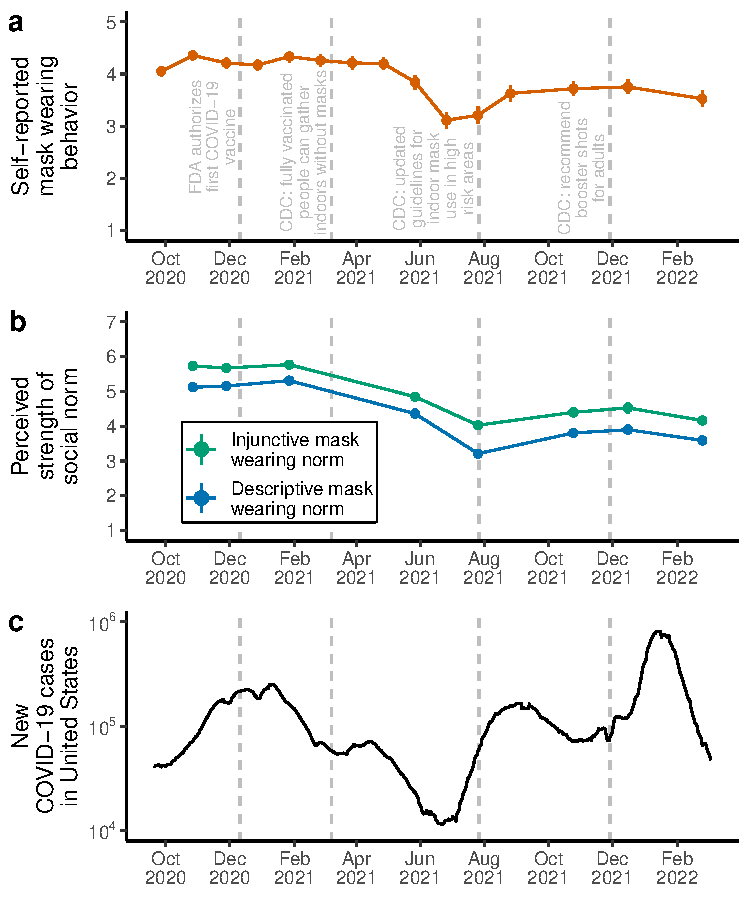
\includegraphics{manuscript_files/figure-latex/plotTimeline-1.pdf}
\caption{\label{fig:plotTimeline}\emph{Timeline of self-reported mask wearing behavior and perceived social norms in the United States throughout the COVID-19 pandemic.} (a) Points and line ranges indicate mean averages and standard errors for the self-reported mask wearing item. This item was measured across all fifteen time points on a 5-point Likert scale, with higher values indicating increased frequency of personal mask wearing during in-person interactions. (b) Points and line ranges indicate mean averages and standard errors for perceived descriptive mask wearing norms (blue) and perceived injunctive mask wearing norms (green). These items were measured across eight time points on a 7-point Likert scale, with higher values indicating stronger perceived social norms. (c) Smoothed data for new COVID-19 cases in the United States, displayed on the log scale (data retrieved from Our World in Data; \url{https://ourworldindata.org/}). Across all panels, gray dashed lines represent significant pandemic-related events in the United States, such as vaccine approval from the Food and Drug Administration (FDA) and public health recommendations from the Centers for Disease Control and Prevention (CDC).}
\end{figure}

Three main observations can be made about the emergence and stability of social norms from these visualizations. First, social norms and behavior were tightly coupled over time. Although social norms are measured on fewer occasions than mask wearing behavior, we can see that as mask wearing behavior decreased in the summer of 2021, so too did perceived descriptive and injunctive mask wearing norms. Subsequently, the steep rise in COVID-19 case numbers in the fall of 2021 saw concomitant increases in both mask wearing behavior and perceived social norms, though to lower levels than before. In line with these patterns, multilevel regression models revealed positive correlations between mask wearing behavior and perceived descriptive mask wearing norms (\emph{b} = 0.25, 95\% confidence interval {[}0.20 0.30{]}) and between mask wearing behavior and perceived injunctive mask wearing norms (\emph{b} = 0.25, 95\% CI {[}0.21 0.30{]}) across individuals and time points (Supplementary Figure \ref{fig:plotCorBehNorm}; Supplementary Table \ref{tab:modelSummaryTable1}).

Second, fluctuations in mask wearing behavior and perceived social norms are in line with recommendations broadcasted by the CDC, the main national public health agency of the United States. We do not have data for the very start of the pandemic in early 2020, but the high levels of mask wearing and strong perceived social norms at the start of our observation window likely emerged after the initial mask wearing recommendation from the CDC in April 2020. Perceived social norms and mask wearing behavior subsequently declined after the CDC rescinded their mask wearing recommendation in March 2021, and then increased again after the CDC updated their guidelines for indoor mask use in high risk areas in August 2021. Impressively, shifts in mask wearing behavior and norms happened on the timescale of weeks. These trends were confirmed by a series of multilevel regression models with change points aligning with changes in CDC mask wearing recommendations (Supplementary Figure \ref{fig:plotCDCSens}; Supplementary Table \ref{tab:changePointsTable}).

Third, across all eight time points with available data, injunctive mask wearing norms were consistently rated as stronger than descriptive mask wearing norms. Multilevel regression modeling revealed that, on average across individuals and time points, injunctive norms were rated as 0.6 points stronger than descriptive norms on a 7-point Likert scale (\emph{b} = 0.60, 95\% CI {[}0.51 0.69{]}; Supplementary Figure \ref{fig:plotNormCompare}; Supplementary Table \ref{tab:modelSummaryTable2}). In other words, participants in our study perceived the general encouragement of mask wearing and mask wearing behavior among trusted people to be higher than perceived mask wearing among people in their local area.

Sample averages can provide informative trends, but they do not allow us to estimate within-person changes in mask wearing behavior and perceived social norms over time. To determine whether within-person changes in social norms temporally preceded within-person changes in mask wearing behavior, we fitted an eight-wave unconstrained random-intercept cross-lagged panel model to the longitudinal data. This structural equation model separately estimated stable trait-like between-person individual differences and within-person fluctuations from trait levels for our three main variables: self-reported mask wearing behavior, perceived descriptive mask wearing norms, and perceived injunctive mask wearing norms (see Supplementary Table \ref{tab:lavaanTable} for estimated model parameters). According to established fit statistics, this model fitted the data well (root mean square error of approximation = 0.037, 95\% CI {[}0.032 0.042{]}; standardized root mean squared residual = 0.056; comparative fit index = 0.961).

Regarding between-person individual differences, the covariances between the random intercepts in the model revealed positive correlations between stable trait levels of mask wearing behavior and perceived social norms. On average across the whole study, participants who more frequently wore masks during in-person interactions also perceived stronger descriptive mask wearing norms (\emph{r} = 0.45, 95\% CI {[}0.35 0.54{]}, \emph{p} \textless{} .001) and stronger injunctive mask wearing norms (\emph{r} = 0.29, 95\% CI {[}0.18 0.40{]}, \emph{p} \textless{} .001). Stable trait perceptions of descriptive and injunctive mask wearing norms were also highly positively correlated (\emph{r} = 0.65, 95\% CI {[}0.58 0.71{]}, \emph{p} \textless{} .001).

Regarding within-person dynamics over time, Figure \ref{fig:plotRICLPM} displays autoregressive and cross-lagged effects for all three variables across the study duration. In random intercept cross-lagged panel models, autoregressive effects represent ``persistence'' or ``inertia'' in within-person fluctuations from stable trait levels. In other words, a positive autoregressive effect indicates that being higher than average on one measure predicts being higher than average on that same measure in the following time point (this is not to be confused with the ``stability'' of the measure over time, which is captured by the random intercepts in our model). By contrast, and most relevant for the current study, cross-lagged effects represent the effect of a within-person fluctuation in one measure on future within-person fluctuations in other measures. In other words, a positive cross-lagged effect indicates that being higher than average on one measure predicts being higher than average on \emph{another} measure in the following time point. Cross-lagged effects are thus used to infer within-person causal influences over time.



\begin{figure}
\centering
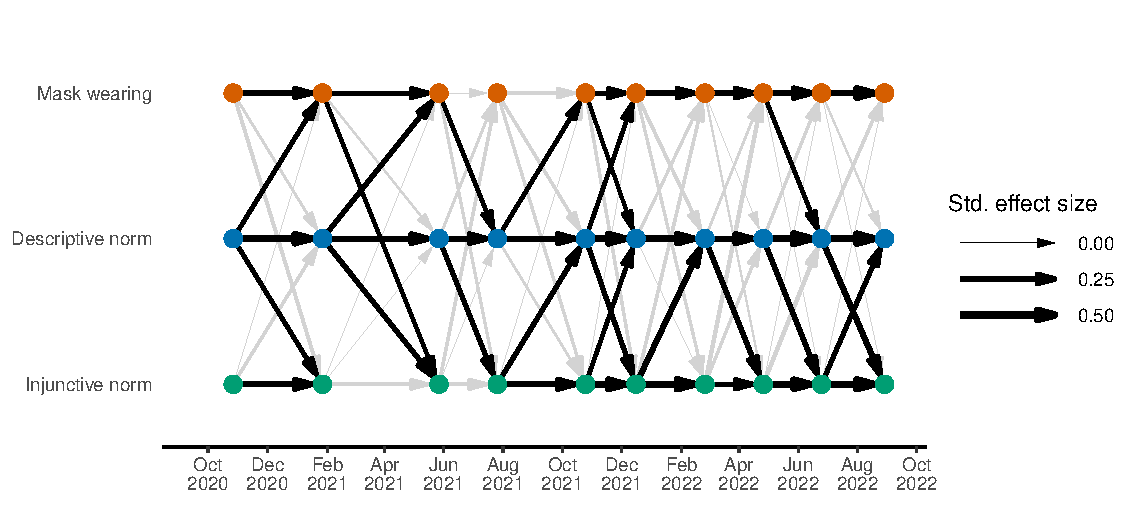
\includegraphics{manuscript_files/figure-latex/plotRICLPM-1.pdf}
\caption{\label{fig:plotRICLPM}\emph{Results of eight-wave unconstrained random-intercept cross-lagged panel model.} Arrows represent within-person autoregressive and cross-lagged effects from the model, controlling for time invariant predictors and partitioning out stable between-person individual differences. Arrow thickness is scaled according to standardized effect size. Bolded arrows indicate significantly positive parameters, \emph{p} \textless{} 0.05. Gray arrows indicate non-significant parameters.}
\end{figure}

Earlier in the pandemic, we see less evidence of autoregressive and cross-lagged effects. Within-person fluctuations in descriptive and injunctive norms persist across only a few time points, and there is only one cross-lagged effect of mask wearing on future descriptive norms. However, once COVID-19 case numbers start rising again in June 2021, we begin to see more evidence of autoregressive and cross-lagged effects. From this point onwards, all three variables show evidence of persistence, with within-person fluctuations from trait levels predicting later within-person fluctuations in the same measures. But more importantly, several positive and significant cross-lagged effects emerge. On three occasions, within-person increases in perceived descriptive norms predicted future within-person increases in mask wearing behavior. According to recent effect size guidelines for cross-lagged panel models (Orth et al., 2022), the standardized beta coefficients for these cross-lagged effects were large (Time 9, \(\beta\) = 0.17, 95\% CI {[}0.03 0.31{]}, \emph{p} = .020; Time 11, \(\beta\) = 0.21, 95\% CI {[}0.06 0.36{]}, \emph{p} = .006; Time 13, \(\beta\) = 0.16, 95\% CI {[}0.01 0.31{]}, \emph{p} = .037). We also find some evidence for a reciprocal effect, whereby within-person increases in mask wearing behavior predicted future within-person increases in perceived descriptive norms. Moreover, several cross-lagged effects emerged between perceived descriptive and injunctive norms, demonstrating reciprocal within-person causal effects between these variables.

However, the model reveals that, after controlling for perceived descriptive norms, within-person changes in perceived injunctive norms were unrelated to within-person changes in mask wearing behavior across the entire pandemic. All cross-lagged effects between the two variables, both from perceived injunctive norms to mask wearing behavior and vice versa, are non-significant. Any causal effect that perceived injunctive norms might have had on future mask wearing behavior appears to be fully mediated by perceived descriptive norms. For example, between August 2021 and December 2021, perceived injunctive norms predicted future perceived descriptive norms, which themselves predicted future mask wearing behavior. But aside from these indirect effects, perceived injunctive norms and mask wearing behavior were not directly causally related over time within individuals.

\hypertarget{discussion}{%
\section{Discussion}\label{discussion}}

Using longitudinal data from the United States across the entire COVID-19 pandemic, we aimed to understand how descriptive and injunctive mask wearing norms emerge and influence behavior in response to a naturally unfolding social dilemma. The trends of norm perceptions and self-reported mask wearing over time suggest that norms and behavior are tightly coupled, and both change quickly in response to recommendations from public health authorities. The results of our structural equation model also indicate that descriptive norms caused future increases in mask wearing behavior from June 2021 onwards. While injunctive norms were perceived as stronger than descriptive norms, we found that injunctive norms were not directly causally related to future mask wearing behavior over the course of the pandemic.

Our finding that social norms and mask wearing behavior are tightly coupled over time provides real-world support for experimental evidence that social norms and cooperative behavior develop synergistically within groups via processes of social interaction (Titlestad et al., 2019). Moreover, the role of authorities, like the CDC, in shaping social norms and behavior supports the idea that institutions are part of the process by which culture and one's own behaviors are mutually constructed (Markus \& Kitayama, 2010). The CDC explicitly releases guidelines for the benefit of public health, one of many situations in which the function of authorities is to coordinate behavior on large scales. However, even when institutions do not intend to coordinate behavior, they still may introduce influential social norms into the population (e.g., through business practices or products produced).

We also found that injunctive norms were, on average, perceived as stronger than descriptive norms. This aligns with previous research that measured perceived injunctive and descriptive norms in the contexts of drinking (Park et al., 2009) and marijuana use (Montes et al., 2021). What people ought to do is often perceived as stronger than what people \emph{actually} do. Since we operationalized injunctive norms in part by whether trusted individuals in the media were wearing masks, it is possible that our sample is accurately reporting that people in general were less adherent to mask wearing policies than government officials, newscasters, and other respected individuals. It may also have been easier for our participants to notice instances of non-compliance with mask wearing guidelines among the general population, simply because they have more opportunities to observe people's behavior in public settings.

Despite perceiving stronger injunctive norms, it was \emph{descriptive} norms, not injunctive norms, that independently predicted future increases in mask wearing. In line with this finding, descriptive norms have also been shown to predict future increases in physical distancing and prosocial behaviors (e.g., neighborhood help, charitable donations) throughout the COVID-19 pandemic, though this previous work did not adequately disentangle between-person and within-person effects (Rudert \& Janke, 2021). Similarly, experimental work has revealed that people in the United States are more likely to report intentions to wear a mask if they are told that others are wearing masks (Bokemper et al., 2021). Why this specific effect of descriptive norms on mask wearing? Descriptive norms are particularly useful for fast changing, threatening situations with a high degree of uncertainty, such as the COVID-19 pandemic (Gelfand \& Harrington, 2015). During times of uncertainty, people look to others to quickly coordinate their behavior, and attempt to alleviate uncertainty-related stress by identifying with their group and its social norms (Hogg et al., 2008; Wellen et al., 1998). Supporting this situational-uncertainty explanation, our model revealed that descriptive norms only began to predict future mask wearing after the CDC flipped their mask wearing recommendation in March 2021. With changing recommendations from authorities increasing levels of uncertainty, people instead began to look to their neighbors and adapted their mask wearing behavior accordingly.

Our finding that injunctive norms do not predict future mask wearing behavior is at odds with cross-sectional evidence showing that perceived injunctive norms are positively correlated with intentions to stay indoors during the pandemic among older adults (Macy et al., 2021). One possible explanation for these conflicting findings is that, due to the increased opportunities to observe mask wearing in public, descriptive norms of mask wearing behavior were made more salient than injunctive norms throughout the pandemic, and therefore had a greater influence on behavior (Cialdini et al., 1991). By contrast, for more private behaviors like remaining indoors, it would have been less possible to observe other people's behaviors, increasing the relative salience of injunctive norms. To test this idea, future research should expand our longitudinal cross-lagged approach to protective behaviors beyond mask wearing, including both public behaviors (e.g., physical distancing) and private behaviors (e.g., hand washing and home isolation).

We are limited in generalizing these findings due to the constraints of our sample and the variables considered. While our sample began as representative of the United States, there was significant attrition over the course of the study (Supplementary Figure \ref{fig:plotAttrition}). This attrition did not leave us with enough data to test the robustness of our results within different identity groups, such as different genders, different ethnicities, or those with different political ideologies. Since injunctive norm strength varies based on which group is seen as the source of the norm (Neighbors et al., 2008), it would be interesting to learn whether different groups have different patterns of norm emergence over time. In particular, future analyses with larger samples should consider political ideology as a group identity, due to the political polarization of COVID-19 protective behaviors (Baxter-King et al., 2022). Our sample was predominantly White, and so future larger samples should be intentionally more diverse, answering calls to avoid generalizing White samples as representative of human behavior at large (Remedios, 2022). Our results also might not generalize to all social norms, behaviors, and social dilemmas. Norms governing sustainability in response to climate change, for example, might take longer to emerge, since the threat of climate change is more abstract and remote than the COVID-19 pandemic. For more distant social dilemmas that do not cause immediate day-to-day uncertainty, descriptive social norms may not necessarily drive cooperative behavior.

Regardless, in the case of mask wearing in the United States over the COVID-19 pandemic, we have shown that social norms developed rapidly in the population and responded to both recommendations from authorities and current levels of cooperative behavior. Moreover, we found that descriptive norms, rather than injunctive norms, were the main driver for future mask wearing. Importantly, this key finding slices both ways. Not only does it imply that high local levels of mask wearing encouraged future personal mask use, but it also implies that \emph{low} local levels of mask wearing \emph{discouraged} future personal mask use. This echoes recent reports of people in the United States not wanting to be ``singled out'' by being the only one wearing a mask in their community (Natanson, 2022). Our work thus underscores the importance of consistent, visible community adherence for encouraging personal protective behaviors in response to global pandemics like COVID-19.

\newpage

\hypertarget{acknowledgements}{%
\section{Acknowledgements}\label{acknowledgements}}

This study was funded by the Interdisciplinary Cooperation Initiative, ASU President's Office, the Cooperation Science Network, the Institute for Mental Health Research, the University of New Mexico, the Indiana University College of Arts \& Sciences, the Rutgers University Center for Human Evolutionary Studies, the Charles Koch Foundation, and the John Templeton Foundation.

\hypertarget{author-contributions}{%
\section{Author Contributions}\label{author-contributions}}

SLH, ERH, and PMT conceptualized the study. SLH and SC oversaw the data curation, investigation, and methodology of the study, and wrote the first draft of the paper. SC conducted the formal analysis and created all visualisations. ERH and PMT provided funding and supervision for the study. All authors reviewed and edited the final draft of the paper.

\hypertarget{conflicts-of-interest}{%
\section{Conflicts of Interest}\label{conflicts-of-interest}}

There are no conflicts of interest to declare.

\hypertarget{research-transparency-and-reproducibility}{%
\section{Research Transparency and Reproducibility}\label{research-transparency-and-reproducibility}}

All data and code to reproduce the statistical analyses in this manuscript can be found on GitHub: \url{https://github.com/ScottClaessens/covidMaskWearing}

\newpage

\hypertarget{references}{%
\section{References}\label{references}}

\begingroup
\setlength{\parindent}{-1in}
\setlength{\leftskip}{0.5in}

\hypertarget{refs}{}
\begin{CSLReferences}{1}{0}
\leavevmode\vadjust pre{\hypertarget{ref-Asch1956}{}}%
Asch, S. E. (1956). Studies of independence and conformity: I. A minority of one against a unanimous majority. \emph{Psychological Monographs: General and Applied}, \emph{70}(9), 1. \url{https://doi.org/10.1037/h0093718}

\leavevmode\vadjust pre{\hypertarget{ref-Aust2022}{}}%
Aust, F., \& Barth, M. (2022). \emph{{papaja}: {Prepare} reproducible {APA} journal articles with {R Markdown}}. \url{https://github.com/crsh/papaja}

\leavevmode\vadjust pre{\hypertarget{ref-Bates2015}{}}%
Bates, D., Mächler, M., Bolker, B., \& Walker, S. (2015). Fitting linear mixed-effects models using lme4. \emph{Journal of Statistical Software}, \emph{67}(1), 1--48. \url{https://doi.org/10.18637/jss.v067.i01}

\leavevmode\vadjust pre{\hypertarget{ref-BaxterKing2022}{}}%
Baxter-King, R., Brown, J. R., Enos, R. D., Naeim, A., \& Vavreck, L. (2022). How local partisan context conditions prosocial behaviors: Mask wearing during {COVID-19}. \emph{Proceedings of the National Academy of Sciences}, \emph{119}(21), e2116311119. \url{https://doi.org/10.1073/pnas.2116311119}

\leavevmode\vadjust pre{\hypertarget{ref-Bokemper2021}{}}%
Bokemper, S. E., Cucciniello, M., Rotesi, T., Pin, P., Malik, A. A., Willebrand, K., Paintsil, E. E., Omer, S. B., Huber, G. A., \& Melegaro, A. (2021). Experimental evidence that changing beliefs about mask efficacy and social norms increase mask wearing for {COVID-19} risk reduction: Results from the {United States} and {Italy}. \emph{PLOS ONE}, \emph{16}(10), e0258282. \url{https://doi.org/10.1371/journal.pone.0258282}

\leavevmode\vadjust pre{\hypertarget{ref-Boyd1985}{}}%
Boyd, \&. R., Robert. (1985). \emph{Culture and the evolutionary process}. University of Chicago Press.

\leavevmode\vadjust pre{\hypertarget{ref-CDC2022b}{}}%
Centers for Disease Control and Prevention. (2022a). \emph{{CDC Museum COVID-19 Timeline}}. \url{https://www.cdc.gov/museum/timeline/covid19.html}

\leavevmode\vadjust pre{\hypertarget{ref-CDC2022a}{}}%
Centers for Disease Control and Prevention. (2022b). \emph{{United States COVID-19 Community Levels by County}} {[}Data set{]}. \url{https://data.cdc.gov/Public-Health-Surveillance/United-States-COVID-19-Community-Levels-by-County/3nnm-4jni}

\leavevmode\vadjust pre{\hypertarget{ref-Cialdini2007}{}}%
Cialdini, R. B. (2007). Descriptive social norms as underappreciated sources of social control. \emph{Psychometrika}, \emph{72}(2), 263--268. \url{https://doi.org/10.1007/s11336-006-1560-6}

\leavevmode\vadjust pre{\hypertarget{ref-Cialdini2021}{}}%
Cialdini, R. B., \& Jacobson, R. P. (2021). Influences of social norms on climate change-related behaviors. \emph{Current Opinion in Behavioral Sciences}, \emph{42}, 1--8. \url{https://doi.org/10.1016/j.cobeha.2021.01.005}

\leavevmode\vadjust pre{\hypertarget{ref-Cialdini1991}{}}%
Cialdini, R. B., Kallgren, C. A., \& Reno, R. R. (1991). \emph{A focus theory of normative conduct: A theoretical refinement and reevaluation of the role of norms in human behavior} (M. P. Zanna, Ed.; Vol. 24, pp. 201--234). Academic Press. \url{https://doi.org/10.1016/S0065-2601(08)60330-5}

\leavevmode\vadjust pre{\hypertarget{ref-Deutsch1955}{}}%
Deutsch, M., \& Gerard, H. B. (1955). A study of normative and informational social influences upon individual judgment. \emph{The Journal of Abnormal and Social Psychology}, \emph{51}(3), 629--636. \url{https://doi.org/10.1037/h0046408}

\leavevmode\vadjust pre{\hypertarget{ref-Fehr2018a}{}}%
Fehr, E., \& Schurtenberger, I. (2018a). Normative foundations of human cooperation. \emph{Nature Human Behaviour}, \emph{2}(7), 458--468. \url{https://doi.org/10.1038/s41562-018-0385-5}

\leavevmode\vadjust pre{\hypertarget{ref-Fehr2018b}{}}%
Fehr, E., \& Schurtenberger, I. (2018b). \emph{The dynamics of norm formation and norm decay} (Working Paper Series). Department of Economics 278, University of Zurich. \url{https://doi.org/10.5167/uzh-147925}

\leavevmode\vadjust pre{\hypertarget{ref-Gelfand2015}{}}%
Gelfand, M. J., \& Harrington, J. R. (2015). The motivational force of descriptive norms: For whom and when are descriptive norms most predictive of behavior? \emph{Journal of Cross-Cultural Psychology}, \emph{46}(10), 1273--1278. \url{https://doi.org/10.1177/0022022115600796}

\leavevmode\vadjust pre{\hypertarget{ref-Gelfand2011}{}}%
Gelfand, M. J., Raver, J. L., Nishii, L., Leslie, L. M., Lun, J., Lim, B. C., Duan, L., Almaliach, A., Ang, S., Arnadottir, J., Aycan, Z., Boehnke, K., Boski, P., Cabecinhas, R., Chan, D., Chhokar, J., D'Amato, A., Ferrer, M., Fischlmayr, I. C., \ldots{} Yamaguchi, S. (2011). Differences between tight and loose cultures: A 33-nation study. \emph{Science}, \emph{332}(6033), 1100--1104. \url{https://doi.org/10.1126/science.1197754}

\leavevmode\vadjust pre{\hypertarget{ref-Goldstein2008}{}}%
Goldstein, N. J., Cialdini, R. B., \& Griskevicius, V. (2008). A room with a viewpoint: Using social norms to motivate environmental conservation in hotels. \emph{Journal of Consumer Research}, \emph{35}(3), 472--482. \url{https://doi.org/10.1086/586910}

\leavevmode\vadjust pre{\hypertarget{ref-Granger1969}{}}%
Granger, C. W. J. (1969). Investigating causal relations by econometric models and cross-spectral methods. \emph{Econometrica}, \emph{37}(3), 424--438. \url{https://doi.org/10.2307/1912791}

\leavevmode\vadjust pre{\hypertarget{ref-Hamaker2015}{}}%
Hamaker, E. L., Kuiper, R. M., \& Grasman, R. P. P. P. (2015). A critique of the cross-lagged panel model. \emph{Psychological Methods}, \emph{20}(1), 102. \url{https://doi.org/10.1037/a0038889}

\leavevmode\vadjust pre{\hypertarget{ref-Henrich2015}{}}%
Henrich, J. (2015). \emph{The secret of our success: How culture is driving human evolution, domesticating our species, and making us smarter}. Princeton University Press.

\leavevmode\vadjust pre{\hypertarget{ref-Hogg2008}{}}%
Hogg, M. A., Hohman, Z. P., \& Rivera, J. E. (2008). Why do people join groups? Three motivational accounts from social psychology. \emph{Social and Personality Psychology Compass}, \emph{2}(3), 1269--1280. \url{https://doi.org/10.1111/j.1751-9004.2008.00099.x}

\leavevmode\vadjust pre{\hypertarget{ref-Jensen2014}{}}%
Jensen, K., Vaish, A., \& Schmidt, M. F. H. (2014). The emergence of human prosociality: Aligning with others through feelings, concerns, and norms. \emph{Frontiers in Psychology}, \emph{5}, 822. \url{https://doi.org/10.3389/fpsyg.2014.00822}

\leavevmode\vadjust pre{\hypertarget{ref-Jordan2009}{}}%
Jordan, F. M., Gray, R. D., Greenhill, S. J., \& Mace, R. (2009). Matrilocal residence is ancestral in austronesian societies. \emph{Proceedings of the Royal Society B: Biological Sciences}, \emph{276}(1664), 1957--1964. \url{https://doi.org/10.1098/rspb.2009.0088}

\leavevmode\vadjust pre{\hypertarget{ref-Kushnick2014}{}}%
Kushnick, G., Gray, R. D., \& Jordan, F. M. (2014). The sequential evolution of land tenure norms. \emph{Evolution and Human Behavior}, \emph{35}(4), 309--318. \url{https://doi.org/10.1016/j.evolhumbehav.2014.03.001}

\leavevmode\vadjust pre{\hypertarget{ref-Landau2021}{}}%
Landau, W. M. (2021). The targets {R} package: A dynamic {M}ake-like function-oriented pipeline toolkit for reproducibility and high-performance computing. \emph{Journal of Open Source Software}, \emph{6}(57), 2959. \url{https://doi.org/10.21105/joss.02959}

\leavevmode\vadjust pre{\hypertarget{ref-Larkin2018}{}}%
Larkin, C., Sanders, M., Andresen, I., \& Algate, F. (2018). \emph{Testing local descriptive norms and salience of enforcement action: A field experiment to increase tax collection} (SSRN Scholarly Paper No. 3167575). \url{https://doi.org/10.2139/ssrn.3167575}

\leavevmode\vadjust pre{\hypertarget{ref-Macy2021}{}}%
Macy, J. T., Owens, C., Mullis, K., \& Middlestadt, S. E. (2021). The role of self-efficacy and injunctive norms in helping older adults decide to stay home during the {COVID-19} pandemic. \emph{Frontiers in Public Health}, \emph{9}, 660813. \url{https://doi.org/10.3389/fpubh.2021.660813}

\leavevmode\vadjust pre{\hypertarget{ref-Markus2010}{}}%
Markus, H. R., \& Kitayama, S. (2010). Cultures and selves: A cycle of mutual constitution. \emph{Perspectives on Psychological Science}, \emph{5}(4), 420--430. \url{https://doi.org/10.1177/1745691610375557}

\leavevmode\vadjust pre{\hypertarget{ref-MITElectionLab}{}}%
MIT Election Data and Science Lab. (2018). \emph{{County Presidential Election Returns 2000-2020}} (Version V10) {[}Data set{]}. {Harvard Dataverse}. \url{https://doi.org/10.7910/DVN/VOQCHQ}

\leavevmode\vadjust pre{\hypertarget{ref-Montes2021}{}}%
Montes, K. S., Richards, D. K., \& Pearson, M. R. (2021). A novel approach to assess descriptive and injunctive norms for college student marijuana use. \emph{Addictive Behaviors}, \emph{117}, 106755. \url{https://doi.org/10.1016/j.addbeh.2020.106755}

\leavevmode\vadjust pre{\hypertarget{ref-Natanson2022}{}}%
Natanson, H. (2022). Peer pressure is ending mask usage in schools. \emph{The Washingston Post}. \url{https://www.washingtonpost.com/education/2022/02/25/peer-pressure-mask-optional-schools/}

\leavevmode\vadjust pre{\hypertarget{ref-Neighbors2008}{}}%
Neighbors, C., O'Connor, R. M., Lewis, M. A., Chawla, N., Lee, C. M., \& Fossos, N. (2008). The relative impact of injunctive norms on college student drinking: The role of reference group. \emph{Psychology of Addictive Behaviors}, \emph{22}(4), 576--581. \url{https://doi.org/10.1037/a0013043}

\leavevmode\vadjust pre{\hypertarget{ref-Nigbur2010}{}}%
Nigbur, D., Lyons, E., \& Uzzell, D. (2010). Attitudes, norms, identity and environmental behaviour: Using an expanded theory of planned behaviour to predict participation in a kerbside recycling programme. \emph{British Journal of Social Psychology}, \emph{49}(2), 259--284. \url{https://doi.org/10.1348/014466609X449395}

\leavevmode\vadjust pre{\hypertarget{ref-Orth2022}{}}%
Orth, U., Meier, L. L., Bühler, J. L., Dapp, L. C., Krauss, S., Messerli, D., \& Robins, R. W. (2022). Effect size guidelines for cross-lagged effects. \emph{Psychological Methods}. \url{https://doi.org/10.1037/met0000499}

\leavevmode\vadjust pre{\hypertarget{ref-Park2009}{}}%
Park, H. S., Klein, K. A., Smith, S., \& Martell, D. (2009). Separating subjective norms, university descriptive and injunctive norms, and {U.S.} Descriptive and injunctive norms for drinking behavior intentions. \emph{Health Communication}, \emph{24}(8), 746--751. \url{https://doi.org/10.1080/10410230903265912}

\leavevmode\vadjust pre{\hypertarget{ref-RCoreTeam}{}}%
R Core Team. (2022). \emph{R: A language and environment for statistical computing}. R Foundation for Statistical Computing. \url{https://www.R-project.org/}

\leavevmode\vadjust pre{\hypertarget{ref-Rakoczy2013}{}}%
Rakoczy, H., \& Schmidt, M. F. H. (2013). The early ontogeny of social norms. \emph{Child Development Perspectives}, \emph{7}(1), 17--21. \url{https://doi.org/10.1111/cdep.12010}

\leavevmode\vadjust pre{\hypertarget{ref-Remedios2022}{}}%
Remedios, J. D. (2022). Psychology must grapple with whiteness. \emph{Nature Reviews Psychology}, \emph{1}(3), 125--126. \url{https://doi.org/10.1038/s44159-022-00024-4}

\leavevmode\vadjust pre{\hypertarget{ref-Rosseel2012}{}}%
Rosseel, Y. (2012). {lavaan}: An {R} package for structural equation modeling. \emph{Journal of Statistical Software}, \emph{48}(2), 1--36. \url{https://doi.org/10.18637/jss.v048.i02}

\leavevmode\vadjust pre{\hypertarget{ref-Rudert2021}{}}%
Rudert, S. C., \& Janke, S. (2021). Following the crowd in times of crisis: Descriptive norms predict physical distancing, stockpiling, and prosocial behavior during the {COVID-19} pandemic. \emph{Group Processes \& Intergroup Relations}, 13684302211023562. \url{https://doi.org/10.1177/13684302211023562}

\leavevmode\vadjust pre{\hypertarget{ref-Schaumberg2022}{}}%
Schaumberg, R. L., \& Skowronek, S. E. (2022). Shame broadcasts social norms: The positive social effects of shame on norm acquisition and normative behavior. \emph{Psychological Science}, 09567976221075303. \url{https://doi.org/10.1177/09567976221075303}

\leavevmode\vadjust pre{\hypertarget{ref-Schmidt2012}{}}%
Schmidt, M. F. H., \& Tomasello, M. (2012). Young children enforce social norms. \emph{Current Directions in Psychological Science}, \emph{21}(4), 232--236. \url{https://doi.org/10.1177/0963721412448659}

\leavevmode\vadjust pre{\hypertarget{ref-Schultz2007}{}}%
Schultz, P. W., Nolan, J. M., Cialdini, R. B., Goldstein, N. J., \& Griskevicius, V. (2007). The constructive, destructive, and reconstructive power of social norms. \emph{Psychological Science}, \emph{18}(5), 429--434. \url{https://doi.org/10.1111/j.1467-9280.2007.01917.x}

\leavevmode\vadjust pre{\hypertarget{ref-Smith2015}{}}%
Smith, L. G. E., Thomas, E. F., \& McGarty, C. (2015). "We must be the change we want to see in the world": Integrating norms and identities through social interaction. \emph{Political Psychology}, \emph{36}(5), 543--557. \url{https://doi.org/10.1111/pops.12180}

\leavevmode\vadjust pre{\hypertarget{ref-Titlestad2019}{}}%
Titlestad, K., Snijders, T. A. B., Durrheim, K., Quayle, M., \& Postmes, T. (2019). The dynamic emergence of cooperative norms in a social dilemma. \emph{Journal of Experimental Social Psychology}, \emph{84}, 103799. \url{https://doi.org/10.1016/j.jesp.2019.03.010}

\leavevmode\vadjust pre{\hypertarget{ref-Tomasello2014}{}}%
Tomasello, M. (2014). The ultra-social animal. \emph{European Journal of Social Psychology}, \emph{44}(3), 187--194. \url{https://doi.org/10.1002/ejsp.2015}

\leavevmode\vadjust pre{\hypertarget{ref-Vaish2011}{}}%
Vaish, A., Carpenter, M., \& Tomasello, M. (2011). Young children's responses to guilt displays. \emph{Developmental Psychology}, \emph{47}(5), 1248--1262. \url{https://doi.org/10.1037/a0024462}

\leavevmode\vadjust pre{\hypertarget{ref-VanKleef2019}{}}%
van Kleef, G. A., Gelfand, M. J., \& Jetten, J. (2019). The dynamic nature of social norms: New perspectives on norm development, impact, violation, and enforcement. \emph{Journal of Experimental Social Psychology}, \emph{84}, 103814. \url{https://doi.org/10.1016/j.jesp.2019.05.002}

\leavevmode\vadjust pre{\hypertarget{ref-Wellen1998}{}}%
Wellen, J. M., Hogg, M. A., \& Terry, D. J. (1998). Group norms and attitude-behavior consistency: The role of group salience and mood. \emph{Group Dynamics: Theory, Research, and Practice}, \emph{2}(1), 48--56. \url{https://doi.org/10.1037/1089-2699.2.1.48}

\leavevmode\vadjust pre{\hypertarget{ref-Wickham2016}{}}%
Wickham, H. (2016). \emph{{ggplot2}: Elegant graphics for data analysis}. Springer-Verlag New York. \url{https://ggplot2.tidyverse.org}

\leavevmode\vadjust pre{\hypertarget{ref-Wilke2020}{}}%
Wilke, C. O. (2020). \emph{{cowplot}: Streamlined plot theme and plot annotations for 'ggplot2'}. \url{https://CRAN.R-project.org/package=cowplot}

\end{CSLReferences}

\endgroup

\newpage

\hypertarget{appendix-appendix}{%
\appendix}


\renewcommand{\appendixname}{\textbf{Supplementary Materials}}
\renewcommand{\thefigure}{S\arabic{figure}} \setcounter{figure}{0}
\renewcommand{\thetable}{S\arabic{table}} \setcounter{table}{0}
\renewcommand{\theequation}{S\arabic{table}} \setcounter{equation}{0}

\hypertarget{section}{%
\section{}\label{section}}

\hypertarget{supplementary-results}{%
\subsection{Supplementary Results}\label{supplementary-results}}

\hypertarget{construct-validity-for-measures-of-perceived-descriptive-and-injunctive-norms}{%
\subsubsection{Construct validity for measures of perceived descriptive and injunctive norms}\label{construct-validity-for-measures-of-perceived-descriptive-and-injunctive-norms}}

To evaluate the construct validity of our measures of perceived descriptive and injunctive norms, at Time 7 we asked participants to rate the extent to which each perceived norm item provided descriptive and injunctive information. For each item, participants were asked whether the item provided information about what people are doing, and whether the item provided information about what people should be doing. Participants responded on a 7-point Likert scale, from (1) Not At All to (7) Very Strongly. For a full list of questions, see Supplementary Table \ref{tab:itemTable}.

Results showed that participants did differentiate the perceived norm items as expected. Participants rated the perceived descriptive norm items as providing more descriptive information than the perceived injunctive norm items, \emph{t}(442) = -7.28, \emph{p} \textless{} .001 (mean descriptive items = 4.75; mean injunctive items = 4.25). By contrast, participants rated the perceived injunctive norm items as providing more injunctive information than the perceived descriptive norm items, \emph{t}(444) = 7.15, \emph{p} \textless{} .001 (mean descriptive items = 5.11; mean injunctive items = 5.54).

\newpage

\hypertarget{supplementary-figures}{%
\subsection{Supplementary Figures}\label{supplementary-figures}}



\begin{figure}
\centering
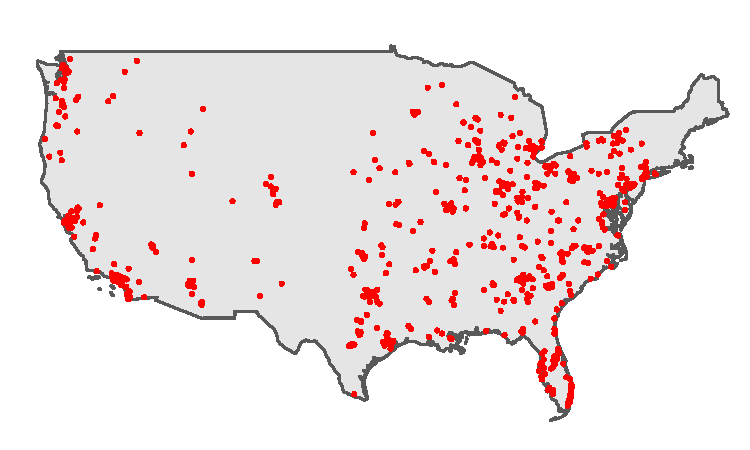
\includegraphics{manuscript_files/figure-latex/plotUSMap-1.pdf}
\caption{\label{fig:plotUSMap}\emph{Map of the United States with participant zip code locations.}}
\end{figure}

\newpage



\begin{figure}
\centering
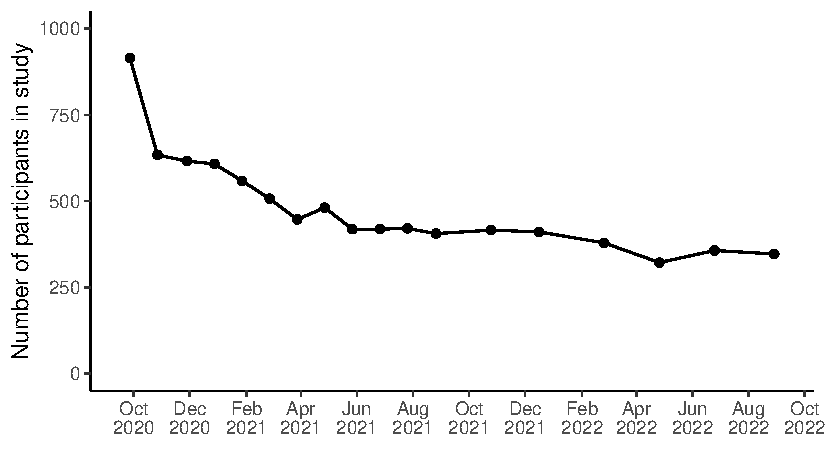
\includegraphics{manuscript_files/figure-latex/plotAttrition-1.pdf}
\caption{\label{fig:plotAttrition}\emph{Attrition across the course of the study.}}
\end{figure}

\newpage



\begin{figure}
\centering
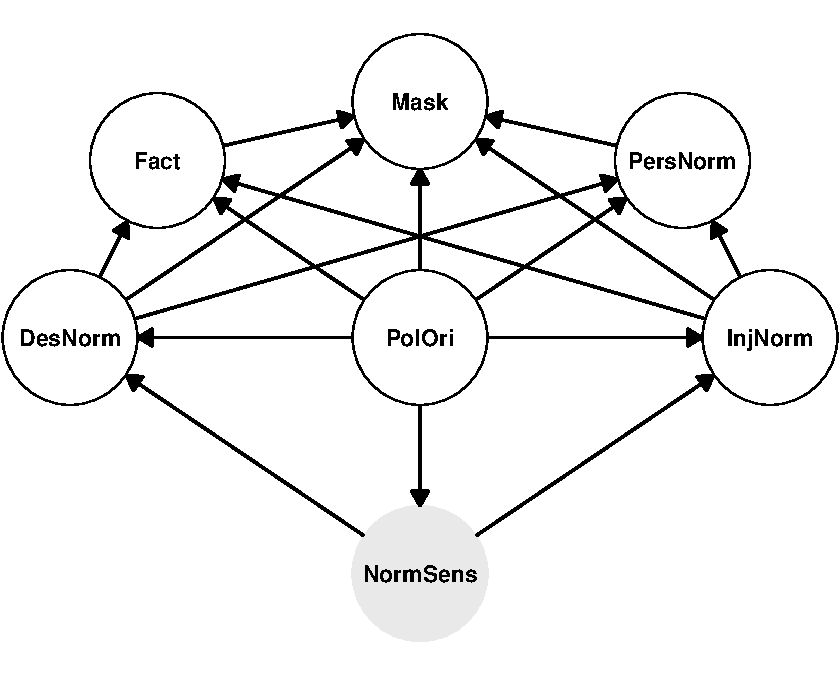
\includegraphics{manuscript_files/figure-latex/plotDAG-1.pdf}
\caption{\label{fig:plotDAG}\emph{Directed acyclic graph reflecting causal assumptions.} In this model, a general unobserved sensitivity to social norms (NormSens) causes perceptions of descriptive social norms (DesNorm) and perceptions of injunctive social norms (InjNorm), and perceptions of descriptive and injunctive norms cause mask wearing behavior (Mask). County-level COVID-19 prevalence (CovidPrev) and political leaning (CountyPol) are also posited to be common causes of perceptions of social norms and mask wearing behavior. Using the backdoor criterion (Pearl, 1995), this causal model implies that it is necessary to control for perceptions of injunctive norms, county-level COVID-19 prevalence, and county-level political leaning to estimate the direct causal effect of perceived descriptive norms on mask wearing. Similarly, it is necessary to control for perceptions of descriptive norms, county-level COVID-19 prevalence, and county-level political leaning to estimate the direct causal effect of perceived injunctive norms on mask wearing.}
\end{figure}

\newpage



\begin{figure}
\centering
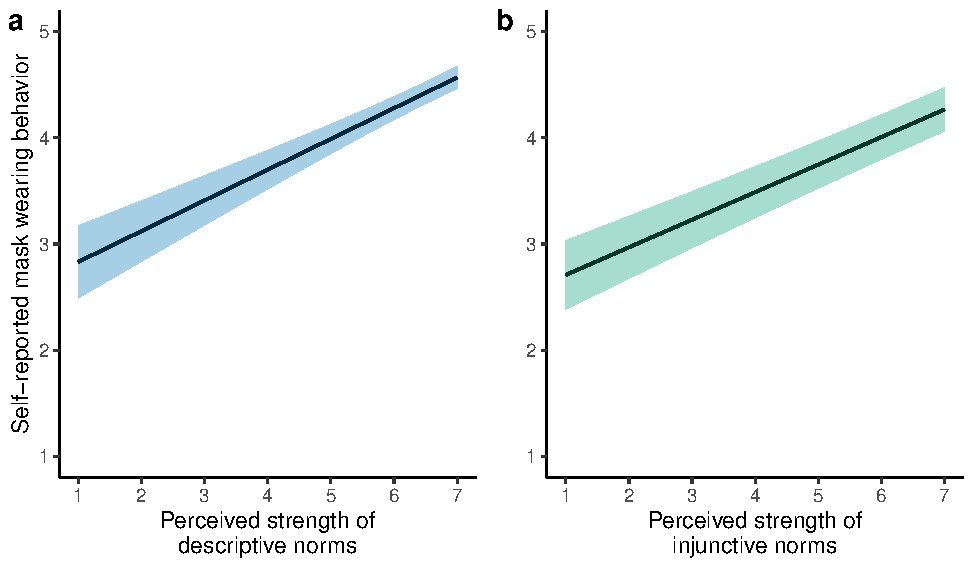
\includegraphics{manuscript_files/figure-latex/plotCorBehNorm-1.pdf}
\caption{\label{fig:plotCorBehNorm}\emph{Predictions from multilevel models with self-reported mask wearing behavior as the outcome variable and (a) perceived strength of descriptive norms and (b) perceived strength of injunctive norms as independent predictor variables.} Lines are fixed effect regression lines from multilevel models, shaded areas are 95\% confidence intervals.}
\end{figure}

\newpage



\begin{figure}
\centering
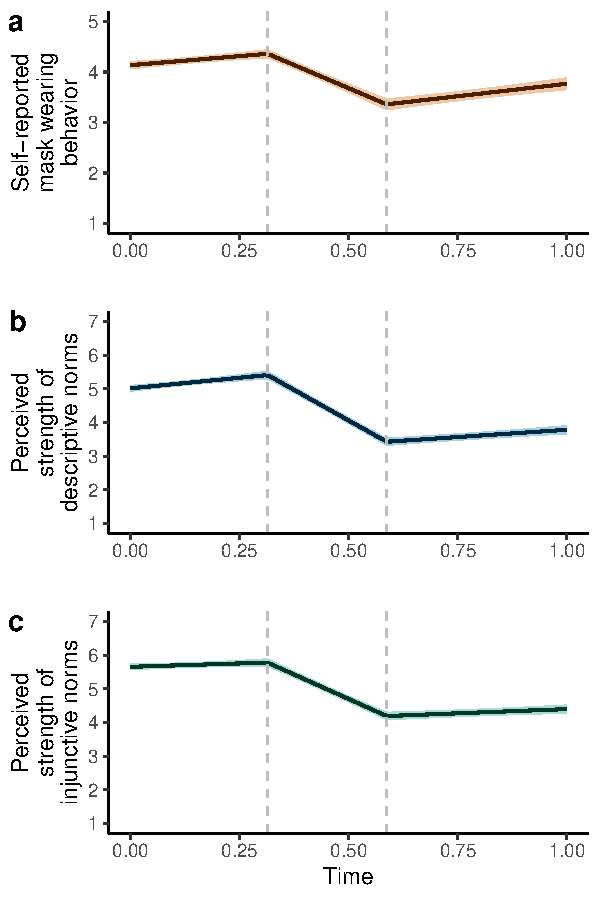
\includegraphics{manuscript_files/figure-latex/plotCDCSens-1.pdf}
\caption{\label{fig:plotCDCSens}\emph{Predictions from multilevel models with change points in line with changes in CDC mask wearing recommendations.} These models track temporal changes in (a) self-reported mask wearing behavior, (b) perceived strength of descriptive norms, and (c) perceived strength of injunctive norms. Time is included as a continuous linear predictor, scaled between 0 and 1, with two forced change points (dashed lines). The first dashed line (left) indicates when the CDC relaxed their mask wearing recommendations in March 2021, and the second dashed line (right) indicates when the CDC strengthened their mask wearing recommendations in July 2021. This results in the estimation of four fixed effect parameters: the initial intercept, the slope in the first window, the slope in the second window, and the slope in the third window. Bolded lines and shaded areas represent fixed effect regression lines from multilevel models and 95\% confidence intervals, respectively.}
\end{figure}

\newpage



\begin{figure}
\centering
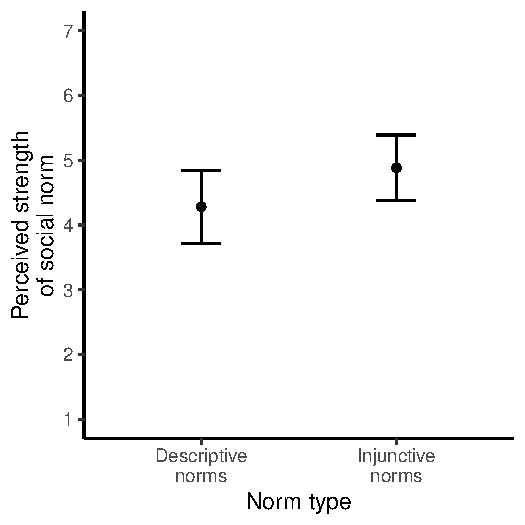
\includegraphics{manuscript_files/figure-latex/plotNormCompare-1.pdf}
\caption{\label{fig:plotNormCompare}\emph{Predictions from multilevel model of the difference between the perceived strength of descriptive and injunctive social norms.} Points and error bars represent estimated marginal means and 95\% confidence intervals, respectively.}
\end{figure}

\newpage

\hypertarget{supplementary-tables}{%
\subsection{Supplementary Tables}\label{supplementary-tables}}



\begin{center}
\begin{ThreePartTable}

\begin{longtable}{m{2.5cm}m{2.5cm}m{9cm}}\noalign{\getlongtablewidth\global\LTcapwidth=\longtablewidth}
\caption{\label{tab:itemTable}List of norm interpretation questions asked at Time 7. \emph{These questions were preceded by the following text:} ``There may or may not be a difference between what people around you are doing and what they should be doing. You can learn about what people are doing and what they should be doing in different ways. For each of the following information sources, we want to know if you can learn from it what people are doing, what people should be doing, or both.'' \emph{Participants answered all questions on a 7-point Likert scale, from (1) Not At All to (7) Very Strongly.}}\\
\toprule
Interpretation & \multicolumn{1}{c}{Perceived norm item} & \multicolumn{1}{c}{Question}\\
\midrule
\endfirsthead
\caption*{\normalfont{Table \ref{tab:itemTable} continued}}\\
\toprule
Interpretation & \multicolumn{1}{c}{Perceived norm item} & \multicolumn{1}{c}{Question}\\
\midrule
\endhead
Provides descriptive information & Descriptive & Does noticing the proportion of people in your area that wear a mask while doing recreational/social activities indoors (e.g., going to the gym, eating at a restaurant, attending a party) tell you what everyone is doing?\\
 &  & Does noticing the proportion of people in your area that wear a mask while doing routine activities indoors (e.g., running errands, shopping, going to work) tell you what everyone is doing?\\
 & Injunctive & Do mask-wearing rules encouraged in your area (e.g., by local or state government officials, businesses, etc.) tell you what everyone is doing?\\
 &  & Does how often you see people that you respect and trust wearing a mask (e.g., on tv, news, etc.) tell you what everyone is doing?\\
Provides injunctive information & Descriptive & Does noticing the proportion of people in your area that wear a mask while doing recreational/social activities indoors (e.g., going to the gym, eating at a restaurant, attending a party) tell you what everyone should be doing?\\
 &  & Does noticing the proportion of people in your area that wear a mask while doing routine activities indoors (e.g., running errands, shopping, going to work) tell you what everyone should be doing?\\
 & Injunctive & Do mask-wearing rules encouraged in your area (e.g., by local or state government officials, businesses, etc.) tell you what everyone should be doing?\\
 &  & Does how often you see people that you respect and trust wearing a mask (e.g., on tv, news, etc.) tell you what everyone should be doing?\\
\bottomrule
\end{longtable}

\end{ThreePartTable}
\end{center}

\newpage



 
  \providecommand{\huxb}[2]{\arrayrulecolor[RGB]{#1}\global\arrayrulewidth=#2pt}
  \providecommand{\huxvb}[2]{\color[RGB]{#1}\vrule width #2pt}
  \providecommand{\huxtpad}[1]{\rule{0pt}{#1}}
  \providecommand{\huxbpad}[1]{\rule[-#1]{0pt}{#1}}

\begin{table}[ht]
\begin{centerbox}
\begin{threeparttable}
\captionsetup{justification=centering,singlelinecheck=off}
\caption{Unstandardized fixed effect parameters from multilevel models: perceptions of social norm strength predicting self-reported mask wearing. \emph{Standard errors are included in brackets.}}
 \label{tab:modelSummaryTable1}
\setlength{\tabcolsep}{0pt}
\begin{tabular}{l l l}


\hhline{>{\huxb{0, 0, 0}{0.8}}->{\huxb{0, 0, 0}{0.8}}->{\huxb{0, 0, 0}{0.8}}-}
\arrayrulecolor{black}

\multicolumn{1}{!{\huxvb{0, 0, 0}{0}}c!{\huxvb{0, 0, 0}{0}}}{\huxtpad{6pt + 1em}\centering \hspace{6pt}  \hspace{6pt}\huxbpad{6pt}} &
\multicolumn{1}{c!{\huxvb{0, 0, 0}{0}}}{\huxtpad{6pt + 1em}\centering \hspace{6pt} Model 1 \hspace{6pt}\huxbpad{6pt}} &
\multicolumn{1}{c!{\huxvb{0, 0, 0}{0}}}{\huxtpad{6pt + 1em}\centering \hspace{6pt} Model 2 \hspace{6pt}\huxbpad{6pt}} \tabularnewline[-0.5pt]


\hhline{>{\huxb{255, 255, 255}{0.4}}->{\huxb{0, 0, 0}{0.4}}->{\huxb{0, 0, 0}{0.4}}-}
\arrayrulecolor{black}

\multicolumn{1}{!{\huxvb{0, 0, 0}{0}}l!{\huxvb{0, 0, 0}{0}}}{\huxtpad{6pt + 1em}\raggedright \hspace{6pt} Intercept \hspace{6pt}\huxbpad{6pt}} &
\multicolumn{1}{r!{\huxvb{0, 0, 0}{0}}}{\huxtpad{6pt + 1em}\raggedleft \hspace{6pt} 2.86\hphantom{0} \hspace{6pt}\huxbpad{6pt}} &
\multicolumn{1}{r!{\huxvb{0, 0, 0}{0}}}{\huxtpad{6pt + 1em}\raggedleft \hspace{6pt} 2.67\hphantom{0} \hspace{6pt}\huxbpad{6pt}} \tabularnewline[-0.5pt]


\hhline{}
\arrayrulecolor{black}

\multicolumn{1}{!{\huxvb{0, 0, 0}{0}}l!{\huxvb{0, 0, 0}{0}}}{\huxtpad{6pt + 1em}\raggedright \hspace{6pt}  \hspace{6pt}\huxbpad{6pt}} &
\multicolumn{1}{r!{\huxvb{0, 0, 0}{0}}}{\huxtpad{6pt + 1em}\raggedleft \hspace{6pt} (0.17) \hspace{6pt}\huxbpad{6pt}} &
\multicolumn{1}{r!{\huxvb{0, 0, 0}{0}}}{\huxtpad{6pt + 1em}\raggedleft \hspace{6pt} (0.16) \hspace{6pt}\huxbpad{6pt}} \tabularnewline[-0.5pt]


\hhline{}
\arrayrulecolor{black}

\multicolumn{1}{!{\huxvb{0, 0, 0}{0}}l!{\huxvb{0, 0, 0}{0}}}{\huxtpad{6pt + 1em}\raggedright \hspace{6pt} Descriptive norms \hspace{6pt}\huxbpad{6pt}} &
\multicolumn{1}{r!{\huxvb{0, 0, 0}{0}}}{\huxtpad{6pt + 1em}\raggedleft \hspace{6pt} 0.25\hphantom{0} \hspace{6pt}\huxbpad{6pt}} &
\multicolumn{1}{r!{\huxvb{0, 0, 0}{0}}}{\huxtpad{6pt + 1em}\raggedleft \hspace{6pt} \hphantom{0}\hphantom{0}\hphantom{0}\hphantom{0} \hspace{6pt}\huxbpad{6pt}} \tabularnewline[-0.5pt]


\hhline{}
\arrayrulecolor{black}

\multicolumn{1}{!{\huxvb{0, 0, 0}{0}}l!{\huxvb{0, 0, 0}{0}}}{\huxtpad{6pt + 1em}\raggedright \hspace{6pt}  \hspace{6pt}\huxbpad{6pt}} &
\multicolumn{1}{r!{\huxvb{0, 0, 0}{0}}}{\huxtpad{6pt + 1em}\raggedleft \hspace{6pt} (0.03) \hspace{6pt}\huxbpad{6pt}} &
\multicolumn{1}{r!{\huxvb{0, 0, 0}{0}}}{\huxtpad{6pt + 1em}\raggedleft \hspace{6pt} \hphantom{0}\hphantom{0}\hphantom{0}\hphantom{0} \hspace{6pt}\huxbpad{6pt}} \tabularnewline[-0.5pt]


\hhline{}
\arrayrulecolor{black}

\multicolumn{1}{!{\huxvb{0, 0, 0}{0}}l!{\huxvb{0, 0, 0}{0}}}{\huxtpad{6pt + 1em}\raggedright \hspace{6pt} Injunctive norms \hspace{6pt}\huxbpad{6pt}} &
\multicolumn{1}{r!{\huxvb{0, 0, 0}{0}}}{\huxtpad{6pt + 1em}\raggedleft \hspace{6pt} \hphantom{0}\hphantom{0}\hphantom{0}\hphantom{0} \hspace{6pt}\huxbpad{6pt}} &
\multicolumn{1}{r!{\huxvb{0, 0, 0}{0}}}{\huxtpad{6pt + 1em}\raggedleft \hspace{6pt} 0.25\hphantom{0} \hspace{6pt}\huxbpad{6pt}} \tabularnewline[-0.5pt]


\hhline{}
\arrayrulecolor{black}

\multicolumn{1}{!{\huxvb{0, 0, 0}{0}}l!{\huxvb{0, 0, 0}{0}}}{\huxtpad{6pt + 1em}\raggedright \hspace{6pt}  \hspace{6pt}\huxbpad{6pt}} &
\multicolumn{1}{r!{\huxvb{0, 0, 0}{0}}}{\huxtpad{6pt + 1em}\raggedleft \hspace{6pt} \hphantom{0}\hphantom{0}\hphantom{0}\hphantom{0} \hspace{6pt}\huxbpad{6pt}} &
\multicolumn{1}{r!{\huxvb{0, 0, 0}{0}}}{\huxtpad{6pt + 1em}\raggedleft \hspace{6pt} (0.02) \hspace{6pt}\huxbpad{6pt}} \tabularnewline[-0.5pt]


\hhline{>{\huxb{255, 255, 255}{0.4}}->{\huxb{0, 0, 0}{0.4}}->{\huxb{0, 0, 0}{0.4}}-}
\arrayrulecolor{black}

\multicolumn{1}{!{\huxvb{0, 0, 0}{0}}l!{\huxvb{0, 0, 0}{0}}}{\huxtpad{6pt + 1em}\raggedright \hspace{6pt} N \hspace{6pt}\huxbpad{6pt}} &
\multicolumn{1}{r!{\huxvb{0, 0, 0}{0}}}{\huxtpad{6pt + 1em}\raggedleft \hspace{6pt} 3781\hphantom{0}\hphantom{0}\hphantom{0}\hphantom{0} \hspace{6pt}\huxbpad{6pt}} &
\multicolumn{1}{r!{\huxvb{0, 0, 0}{0}}}{\huxtpad{6pt + 1em}\raggedleft \hspace{6pt} 3790\hphantom{0}\hphantom{0}\hphantom{0}\hphantom{0} \hspace{6pt}\huxbpad{6pt}} \tabularnewline[-0.5pt]


\hhline{}
\arrayrulecolor{black}

\multicolumn{1}{!{\huxvb{0, 0, 0}{0}}l!{\huxvb{0, 0, 0}{0}}}{\huxtpad{6pt + 1em}\raggedright \hspace{6pt} N (id) \hspace{6pt}\huxbpad{6pt}} &
\multicolumn{1}{r!{\huxvb{0, 0, 0}{0}}}{\huxtpad{6pt + 1em}\raggedleft \hspace{6pt}     778\hphantom{0}\hphantom{0}\hphantom{0}\hphantom{0} \hspace{6pt}\huxbpad{6pt}} &
\multicolumn{1}{r!{\huxvb{0, 0, 0}{0}}}{\huxtpad{6pt + 1em}\raggedleft \hspace{6pt}     778\hphantom{0}\hphantom{0}\hphantom{0}\hphantom{0} \hspace{6pt}\huxbpad{6pt}} \tabularnewline[-0.5pt]


\hhline{}
\arrayrulecolor{black}

\multicolumn{1}{!{\huxvb{0, 0, 0}{0}}l!{\huxvb{0, 0, 0}{0}}}{\huxtpad{6pt + 1em}\raggedright \hspace{6pt} N (time) \hspace{6pt}\huxbpad{6pt}} &
\multicolumn{1}{r!{\huxvb{0, 0, 0}{0}}}{\huxtpad{6pt + 1em}\raggedleft \hspace{6pt}       8\hphantom{0}\hphantom{0}\hphantom{0}\hphantom{0} \hspace{6pt}\huxbpad{6pt}} &
\multicolumn{1}{r!{\huxvb{0, 0, 0}{0}}}{\huxtpad{6pt + 1em}\raggedleft \hspace{6pt}       8\hphantom{0}\hphantom{0}\hphantom{0}\hphantom{0} \hspace{6pt}\huxbpad{6pt}} \tabularnewline[-0.5pt]


\hhline{}
\arrayrulecolor{black}

\multicolumn{1}{!{\huxvb{0, 0, 0}{0}}l!{\huxvb{0, 0, 0}{0}}}{\huxtpad{6pt + 1em}\raggedright \hspace{6pt} AIC \hspace{6pt}\huxbpad{6pt}} &
\multicolumn{1}{r!{\huxvb{0, 0, 0}{0}}}{\huxtpad{6pt + 1em}\raggedleft \hspace{6pt} 11995.16\hphantom{0} \hspace{6pt}\huxbpad{6pt}} &
\multicolumn{1}{r!{\huxvb{0, 0, 0}{0}}}{\huxtpad{6pt + 1em}\raggedleft \hspace{6pt} 12031.84\hphantom{0} \hspace{6pt}\huxbpad{6pt}} \tabularnewline[-0.5pt]


\hhline{}
\arrayrulecolor{black}

\multicolumn{1}{!{\huxvb{0, 0, 0}{0}}l!{\huxvb{0, 0, 0}{0}}}{\huxtpad{6pt + 1em}\raggedright \hspace{6pt} BIC \hspace{6pt}\huxbpad{6pt}} &
\multicolumn{1}{r!{\huxvb{0, 0, 0}{0}}}{\huxtpad{6pt + 1em}\raggedleft \hspace{6pt} 12051.30\hphantom{0} \hspace{6pt}\huxbpad{6pt}} &
\multicolumn{1}{r!{\huxvb{0, 0, 0}{0}}}{\huxtpad{6pt + 1em}\raggedleft \hspace{6pt} 12088.00\hphantom{0} \hspace{6pt}\huxbpad{6pt}} \tabularnewline[-0.5pt]


\hhline{}
\arrayrulecolor{black}

\multicolumn{1}{!{\huxvb{0, 0, 0}{0}}l!{\huxvb{0, 0, 0}{0}}}{\huxtpad{6pt + 1em}\raggedright \hspace{6pt} R2 (fixed) \hspace{6pt}\huxbpad{6pt}} &
\multicolumn{1}{r!{\huxvb{0, 0, 0}{0}}}{\huxtpad{6pt + 1em}\raggedleft \hspace{6pt} 0.07\hphantom{0} \hspace{6pt}\huxbpad{6pt}} &
\multicolumn{1}{r!{\huxvb{0, 0, 0}{0}}}{\huxtpad{6pt + 1em}\raggedleft \hspace{6pt} 0.08\hphantom{0} \hspace{6pt}\huxbpad{6pt}} \tabularnewline[-0.5pt]


\hhline{}
\arrayrulecolor{black}

\multicolumn{1}{!{\huxvb{0, 0, 0}{0}}l!{\huxvb{0, 0, 0}{0}}}{\huxtpad{6pt + 1em}\raggedright \hspace{6pt} R2 (total) \hspace{6pt}\huxbpad{6pt}} &
\multicolumn{1}{r!{\huxvb{0, 0, 0}{0}}}{\huxtpad{6pt + 1em}\raggedleft \hspace{6pt} 0.42\hphantom{0} \hspace{6pt}\huxbpad{6pt}} &
\multicolumn{1}{r!{\huxvb{0, 0, 0}{0}}}{\huxtpad{6pt + 1em}\raggedleft \hspace{6pt} 0.42\hphantom{0} \hspace{6pt}\huxbpad{6pt}} \tabularnewline[-0.5pt]


\hhline{>{\huxb{0, 0, 0}{0.8}}->{\huxb{0, 0, 0}{0.8}}->{\huxb{0, 0, 0}{0.8}}-}
\arrayrulecolor{black}
\end{tabular}
\end{threeparttable}\par\end{centerbox}

\end{table}
 

\newpage



\begin{center}
\begin{ThreePartTable}

\begin{longtable}{lccc}\noalign{\getlongtablewidth\global\LTcapwidth=\longtablewidth}
\caption{\label{tab:changePointsTable}Unstandardized fixed effect parameters from multilevel models: trends over time with change points at CDC events.}\\
\toprule
  & \multicolumn{1}{c}{Mask wearing} & \multicolumn{1}{c}{Descriptive norms} & \multicolumn{1}{c}{Injunctive norms}\\
\midrule
\endfirsthead
\caption*{\normalfont{Table \ref{tab:changePointsTable} continued}}\\
\toprule
  & \multicolumn{1}{c}{Mask wearing} & \multicolumn{1}{c}{Descriptive norms} & \multicolumn{1}{c}{Injunctive norms}\\
\midrule
\endhead
Intercept & 4.13, 95\% CI [4.06 4.21] & 5.01, 95\% CI [4.93 5.10] & 5.65, 95\% CI [5.56 5.75]\\
Slope1 & 0.71, 95\% CI [0.40 1.04] & 1.26, 95\% CI [0.76 1.74] & 0.41, 95\% CI [-0.06 0.90]\\
Slope2 & -3.67, 95\% CI [-4.13 -3.24] & -7.26, 95\% CI [-7.78 -6.75] & -5.82, 95\% CI [-6.37 -5.31]\\
Slope3 & 0.99, 95\% CI [0.69 1.31] & 0.86, 95\% CI [0.56 1.16] & 0.51, 95\% CI [0.21 0.81]\\
N & 7493 & 3837 & 3843\\
R2 (fixed) & 0.05 & 0.26 & 0.21\\
R2 (total) & 0.44 & 0.72 & 0.71\\
\bottomrule
\end{longtable}

\end{ThreePartTable}
\end{center}

\newpage



 
  \providecommand{\huxb}[2]{\arrayrulecolor[RGB]{#1}\global\arrayrulewidth=#2pt}
  \providecommand{\huxvb}[2]{\color[RGB]{#1}\vrule width #2pt}
  \providecommand{\huxtpad}[1]{\rule{0pt}{#1}}
  \providecommand{\huxbpad}[1]{\rule[-#1]{0pt}{#1}}

\begin{table}[ht]
\begin{centerbox}
\begin{threeparttable}
\captionsetup{justification=centering,singlelinecheck=off}
\caption{Unstandardized fixed effect parameters from multilevel model: difference between perceived strength of descriptive and injunctive social norms. \emph{Standard errors are included in brackets.}}
 \label{tab:modelSummaryTable2}
\setlength{\tabcolsep}{0pt}
\begin{tabular}{l l}


\hhline{>{\huxb{0, 0, 0}{0.8}}->{\huxb{0, 0, 0}{0.8}}-}
\arrayrulecolor{black}

\multicolumn{1}{!{\huxvb{0, 0, 0}{0}}c!{\huxvb{0, 0, 0}{0}}}{\huxtpad{6pt + 1em}\centering \hspace{6pt}  \hspace{6pt}\huxbpad{6pt}} &
\multicolumn{1}{c!{\huxvb{0, 0, 0}{0}}}{\huxtpad{6pt + 1em}\centering \hspace{6pt} Model 1 \hspace{6pt}\huxbpad{6pt}} \tabularnewline[-0.5pt]


\hhline{>{\huxb{255, 255, 255}{0.4}}->{\huxb{0, 0, 0}{0.4}}-}
\arrayrulecolor{black}

\multicolumn{1}{!{\huxvb{0, 0, 0}{0}}l!{\huxvb{0, 0, 0}{0}}}{\huxtpad{6pt + 1em}\raggedright \hspace{6pt} Intercept \hspace{6pt}\huxbpad{6pt}} &
\multicolumn{1}{r!{\huxvb{0, 0, 0}{0}}}{\huxtpad{6pt + 1em}\raggedleft \hspace{6pt} 4.28\hphantom{0} \hspace{6pt}\huxbpad{6pt}} \tabularnewline[-0.5pt]


\hhline{}
\arrayrulecolor{black}

\multicolumn{1}{!{\huxvb{0, 0, 0}{0}}l!{\huxvb{0, 0, 0}{0}}}{\huxtpad{6pt + 1em}\raggedright \hspace{6pt}  \hspace{6pt}\huxbpad{6pt}} &
\multicolumn{1}{r!{\huxvb{0, 0, 0}{0}}}{\huxtpad{6pt + 1em}\raggedleft \hspace{6pt} (0.29) \hspace{6pt}\huxbpad{6pt}} \tabularnewline[-0.5pt]


\hhline{}
\arrayrulecolor{black}

\multicolumn{1}{!{\huxvb{0, 0, 0}{0}}l!{\huxvb{0, 0, 0}{0}}}{\huxtpad{6pt + 1em}\raggedright \hspace{6pt} Difference between norm types \hspace{6pt}\huxbpad{6pt}} &
\multicolumn{1}{r!{\huxvb{0, 0, 0}{0}}}{\huxtpad{6pt + 1em}\raggedleft \hspace{6pt} 0.60\hphantom{0} \hspace{6pt}\huxbpad{6pt}} \tabularnewline[-0.5pt]


\hhline{}
\arrayrulecolor{black}

\multicolumn{1}{!{\huxvb{0, 0, 0}{0}}l!{\huxvb{0, 0, 0}{0}}}{\huxtpad{6pt + 1em}\raggedright \hspace{6pt}  \hspace{6pt}\huxbpad{6pt}} &
\multicolumn{1}{r!{\huxvb{0, 0, 0}{0}}}{\huxtpad{6pt + 1em}\raggedleft \hspace{6pt} (0.04) \hspace{6pt}\huxbpad{6pt}} \tabularnewline[-0.5pt]


\hhline{>{\huxb{255, 255, 255}{0.4}}->{\huxb{0, 0, 0}{0.4}}-}
\arrayrulecolor{black}

\multicolumn{1}{!{\huxvb{0, 0, 0}{0}}l!{\huxvb{0, 0, 0}{0}}}{\huxtpad{6pt + 1em}\raggedright \hspace{6pt} N \hspace{6pt}\huxbpad{6pt}} &
\multicolumn{1}{r!{\huxvb{0, 0, 0}{0}}}{\huxtpad{6pt + 1em}\raggedleft \hspace{6pt} 7680\hphantom{0}\hphantom{0}\hphantom{0}\hphantom{0} \hspace{6pt}\huxbpad{6pt}} \tabularnewline[-0.5pt]


\hhline{}
\arrayrulecolor{black}

\multicolumn{1}{!{\huxvb{0, 0, 0}{0}}l!{\huxvb{0, 0, 0}{0}}}{\huxtpad{6pt + 1em}\raggedright \hspace{6pt} N (id) \hspace{6pt}\huxbpad{6pt}} &
\multicolumn{1}{r!{\huxvb{0, 0, 0}{0}}}{\huxtpad{6pt + 1em}\raggedleft \hspace{6pt}     779\hphantom{0}\hphantom{0}\hphantom{0}\hphantom{0} \hspace{6pt}\huxbpad{6pt}} \tabularnewline[-0.5pt]


\hhline{}
\arrayrulecolor{black}

\multicolumn{1}{!{\huxvb{0, 0, 0}{0}}l!{\huxvb{0, 0, 0}{0}}}{\huxtpad{6pt + 1em}\raggedright \hspace{6pt} N (time) \hspace{6pt}\huxbpad{6pt}} &
\multicolumn{1}{r!{\huxvb{0, 0, 0}{0}}}{\huxtpad{6pt + 1em}\raggedleft \hspace{6pt}       8\hphantom{0}\hphantom{0}\hphantom{0}\hphantom{0} \hspace{6pt}\huxbpad{6pt}} \tabularnewline[-0.5pt]


\hhline{}
\arrayrulecolor{black}

\multicolumn{1}{!{\huxvb{0, 0, 0}{0}}l!{\huxvb{0, 0, 0}{0}}}{\huxtpad{6pt + 1em}\raggedright \hspace{6pt} AIC \hspace{6pt}\huxbpad{6pt}} &
\multicolumn{1}{r!{\huxvb{0, 0, 0}{0}}}{\huxtpad{6pt + 1em}\raggedleft \hspace{6pt} 22409.98\hphantom{0} \hspace{6pt}\huxbpad{6pt}} \tabularnewline[-0.5pt]


\hhline{}
\arrayrulecolor{black}

\multicolumn{1}{!{\huxvb{0, 0, 0}{0}}l!{\huxvb{0, 0, 0}{0}}}{\huxtpad{6pt + 1em}\raggedright \hspace{6pt} BIC \hspace{6pt}\huxbpad{6pt}} &
\multicolumn{1}{r!{\huxvb{0, 0, 0}{0}}}{\huxtpad{6pt + 1em}\raggedleft \hspace{6pt} 22472.50\hphantom{0} \hspace{6pt}\huxbpad{6pt}} \tabularnewline[-0.5pt]


\hhline{}
\arrayrulecolor{black}

\multicolumn{1}{!{\huxvb{0, 0, 0}{0}}l!{\huxvb{0, 0, 0}{0}}}{\huxtpad{6pt + 1em}\raggedright \hspace{6pt} R2 (fixed) \hspace{6pt}\huxbpad{6pt}} &
\multicolumn{1}{r!{\huxvb{0, 0, 0}{0}}}{\huxtpad{6pt + 1em}\raggedleft \hspace{6pt} 0.04\hphantom{0} \hspace{6pt}\huxbpad{6pt}} \tabularnewline[-0.5pt]


\hhline{}
\arrayrulecolor{black}

\multicolumn{1}{!{\huxvb{0, 0, 0}{0}}l!{\huxvb{0, 0, 0}{0}}}{\huxtpad{6pt + 1em}\raggedright \hspace{6pt} R2 (total) \hspace{6pt}\huxbpad{6pt}} &
\multicolumn{1}{r!{\huxvb{0, 0, 0}{0}}}{\huxtpad{6pt + 1em}\raggedleft \hspace{6pt} 0.65\hphantom{0} \hspace{6pt}\huxbpad{6pt}} \tabularnewline[-0.5pt]


\hhline{>{\huxb{0, 0, 0}{0.8}}->{\huxb{0, 0, 0}{0.8}}-}
\arrayrulecolor{black}
\end{tabular}
\end{threeparttable}\par\end{centerbox}

\end{table}
 

\newpage





\begin{center}
\begin{ThreePartTable}

\begin{longtable}{lcccc}\noalign{\getlongtablewidth\global\LTcapwidth=\longtablewidth}
\caption{\label{tab:lavaanTable}Standardised autoregressive and cross-lagged parameters from random-intercept cross-lagged panel model. \emph{Variable name prefixes: Mask = mask wearing, Des = perceived descriptive norms, Inj = perceived injunctive norms. Variable name suffixes indicate time points. Arrows indicate the direction of prediction.}}\\
\toprule
Parameter & \multicolumn{1}{c}{Estimate} & \multicolumn{1}{c}{SE} & \multicolumn{1}{c}{2.5\%} & \multicolumn{1}{c}{97.5\%}\\
\midrule
\endfirsthead
\caption*{\normalfont{Table \ref{tab:lavaanTable} continued}}\\
\toprule
Parameter & \multicolumn{1}{c}{Estimate} & \multicolumn{1}{c}{SE} & \multicolumn{1}{c}{2.5\%} & \multicolumn{1}{c}{97.5\%}\\
\midrule
\endhead
Des\_02 → Mask\_03 & -0.01 & 0.06 & -0.14 & 0.11\\
Des\_02 → Inj\_03 & 0.08 & 0.07 & -0.05 & 0.21\\
Des\_02 → Des\_03 & 0.20 & 0.07 & 0.07 & 0.33\\
Des\_03 → Mask\_05 & 0.11 & 0.06 & -0.01 & 0.24\\
Des\_03 → Inj\_05 & 0.10 & 0.07 & -0.03 & 0.23\\
Des\_03 → Des\_05 & 0.32 & 0.06 & 0.19 & 0.44\\
Des\_05 → Mask\_09 & 0.11 & 0.07 & -0.03 & 0.24\\
Des\_05 → Inj\_09 & 0.11 & 0.07 & -0.02 & 0.25\\
Des\_05 → Des\_09 & 0.06 & 0.07 & -0.08 & 0.20\\
Des\_09 → Mask\_11 & 0.17 & 0.07 & 0.03 & 0.31\\
Des\_09 → Inj\_11 & 0.28 & 0.07 & 0.15 & 0.41\\
Des\_09 → Des\_11 & 0.27 & 0.07 & 0.14 & 0.40\\
Des\_11 → Mask\_13 & 0.21 & 0.08 & 0.06 & 0.36\\
Des\_11 → Inj\_13 & 0.15 & 0.07 & 0.01 & 0.30\\
Des\_11 → Des\_13 & 0.27 & 0.07 & 0.13 & 0.41\\
Des\_13 → Mask\_14 & 0.16 & 0.08 & 0.01 & 0.31\\
Des\_13 → Inj\_14 & 0.21 & 0.06 & 0.09 & 0.33\\
Des\_13 → Des\_14 & 0.32 & 0.06 & 0.20 & 0.45\\
Des\_14 → Mask\_15 & 0.15 & 0.08 & -0.02 & 0.31\\
Des\_14 → Inj\_15 & 0.11 & 0.07 & -0.03 & 0.26\\
Des\_14 → Des\_15 & 0.35 & 0.07 & 0.22 & 0.48\\
Inj\_02 → Mask\_03 & 0.10 & 0.06 & -0.02 & 0.23\\
Inj\_02 → Inj\_03 & 0.07 & 0.07 & -0.06 & 0.21\\
Inj\_02 → Des\_03 & 0.03 & 0.06 & -0.09 & 0.15\\
Inj\_03 → Mask\_05 & 0.03 & 0.06 & -0.09 & 0.16\\
Inj\_03 → Inj\_05 & 0.14 & 0.07 & 0.01 & 0.28\\
Inj\_03 → Des\_05 & 0.01 & 0.06 & -0.11 & 0.14\\
Inj\_05 → Mask\_09 & -0.11 & 0.07 & -0.24 & 0.02\\
Inj\_05 → Inj\_09 & -0.07 & 0.07 & -0.21 & 0.07\\
Inj\_05 → Des\_09 & -0.05 & 0.07 & -0.19 & 0.08\\
Inj\_09 → Mask\_11 & 0.04 & 0.08 & -0.11 & 0.19\\
Inj\_09 → Inj\_11 & 0.13 & 0.07 & 0.00 & 0.27\\
Inj\_09 → Des\_11 & 0.07 & 0.07 & -0.06 & 0.21\\
Inj\_11 → Mask\_13 & 0.05 & 0.07 & -0.09 & 0.19\\
Inj\_11 → Inj\_13 & 0.32 & 0.07 & 0.19 & 0.45\\
Inj\_11 → Des\_13 & 0.22 & 0.07 & 0.08 & 0.35\\
Inj\_13 → Mask\_14 & -0.02 & 0.07 & -0.17 & 0.12\\
Inj\_13 → Inj\_14 & 0.42 & 0.06 & 0.31 & 0.54\\
Inj\_13 → Des\_14 & 0.23 & 0.06 & 0.10 & 0.35\\
Inj\_14 → Mask\_15 & 0.03 & 0.08 & -0.13 & 0.18\\
Inj\_14 → Inj\_15 & 0.47 & 0.07 & 0.34 & 0.60\\
Inj\_14 → Des\_15 & 0.31 & 0.06 & 0.19 & 0.44\\
Mask\_02 → Mask\_03 & -0.02 & 0.06 & -0.14 & 0.10\\
Mask\_02 → Inj\_03 & 0.00 & 0.06 & -0.13 & 0.12\\
Mask\_02 → Des\_03 & 0.01 & 0.06 & -0.11 & 0.12\\
Mask\_03 → Mask\_05 & 0.02 & 0.06 & -0.10 & 0.13\\
Mask\_03 → Inj\_05 & 0.04 & 0.06 & -0.08 & 0.16\\
Mask\_03 → Des\_05 & 0.12 & 0.06 & 0.00 & 0.23\\
Mask\_05 → Mask\_09 & 0.08 & 0.07 & -0.04 & 0.21\\
Mask\_05 → Inj\_09 & 0.10 & 0.07 & -0.03 & 0.23\\
Mask\_05 → Des\_09 & -0.01 & 0.07 & -0.15 & 0.12\\
Mask\_09 → Mask\_11 & -0.03 & 0.07 & -0.16 & 0.10\\
Mask\_09 → Inj\_11 & 0.01 & 0.06 & -0.11 & 0.14\\
Mask\_09 → Des\_11 & 0.10 & 0.06 & -0.02 & 0.22\\
Mask\_11 → Mask\_13 & 0.20 & 0.06 & 0.07 & 0.32\\
Mask\_11 → Inj\_13 & 0.05 & 0.06 & -0.07 & 0.16\\
Mask\_11 → Des\_13 & 0.10 & 0.06 & -0.02 & 0.21\\
Mask\_13 → Mask\_14 & 0.30 & 0.06 & 0.18 & 0.42\\
Mask\_13 → Inj\_14 & 0.10 & 0.05 & -0.01 & 0.20\\
Mask\_13 → Des\_14 & 0.20 & 0.05 & 0.09 & 0.30\\
Mask\_14 → Mask\_15 & 0.29 & 0.06 & 0.17 & 0.41\\
Mask\_14 → Inj\_15 & 0.04 & 0.06 & -0.07 & 0.16\\
Mask\_14 → Des\_15 & 0.11 & 0.05 & 0.01 & 0.21\\
\bottomrule
\end{longtable}

\end{ThreePartTable}
\end{center}

\newpage

\hypertarget{supplementary-references}{%
\subsection{Supplementary References}\label{supplementary-references}}

Pearl, J. (1995). Causal diagrams for empirical research. \emph{Biometrika}, \emph{82}(4), 669--688, \url{https://doi.org/10.1093/biomet/82.4.669}


\end{document}
